%% This is file `DEMO-TUDaBeamer.tex' version 3.10 (2021/02/22),
%% it is part of
%% TUDa-CI -- Corporate Design for TU Darmstadt
%% ----------------------------------------------------------------------------
%%
%%  Copyright (C) 2018--2021 by Marei Peischl <marei@peitex.de>
%%
%% ============================================================================
%% This work may be distributed and/or modified under the
%% conditions of the LaTeX Project Public License, either version 1.3c
%% of this license or (at your option) any later version.
%% The latest version of this license is in
%% http://www.latex-project.org/lppl.txt
%% and version 1.3c or later is part of all distributions of LaTeX
%% version 2008/05/04 or later.
%%
%% This work has the LPPL maintenance status `maintained'.
%%
%% The Current Maintainers of this work are
%%   Marei Peischl <tuda-ci@peitex.de>
%%   Markus Lazanowski <latex@ce.tu-darmstadt.de>
%%
%% The development respository can be found at
%% https://github.com/tudace/tuda_latex_templates
%% Please use the issue tracker for feedback!
%%
%% If you need a compiled version of this document, have a look at
%% http://mirror.ctan.org/macros/latex/contrib/tuda-ci/doc
%% or at the documentation directory of this package (if installed)
%% <path to your LaTeX distribution>/doc/latex/tuda-ci
%% ============================================================================
%%
% !TeX program = lualatex
%%

%% This is file `DEMO-TUDaBeamer.tex' version 3.10 (2021/02/22),
%marschall@mma.tu-darmstadt.de% it is part of
%% TUDa-CI -- Corporate Design for TU Darmstadt
%% ----------------------------------------------------------------------------
%%
%%  Copyright (C) 2018--2021 by Marei Peischl <marei@peitex.de>
%%
%% ============================================================================
%% This work may be distributed and/or modified under the
%% conditions of the LaTeX Project Public License, either version 1.3c
%% of this license or (at your option) any later version.
%% The latest version of this license is in
%% http://www.latex-project.org/lppl.txt
%% and version 1.3c or later is part of all distributions of LaTeX
%% version 2008/05/04 or later.
%%
%% This work has the LPPL maintenance status `maintained'.
%%
%% The Current Maintainers of this work are
%%   Marei Peischl <tuda-ci@peitex.de>
%%   Markus Lazanowski <latex@ce.tu-darmstadt.de>
%%
%% The development respository can be found at
%% https://github.com/tudace/tuda_latex_templates
%% Please use the issue tracker for feedback!
%%
%% If you need a compiled version of this document, have a look at
%% http://mirror.ctan.org/macros/latex/contrib/tuda-ci
%% ============================================================================
%%
% !TeX program = lualatex
%%

\documentclass[
	%ngerman,%globale Übergabe der Hauptsprache
	aspectratio=169,%Beamer eigene Option zum Umschalten des Formates
	color={accentcolor=2d},
	logo=true,%Kein Logo auf Folgeseiten
	colorframetitle=true,%Akzentfarbe auch im Frametitle
%	logofile=example-image, %Falls die Logo Dateien nicht vorliegen
	]{tudabeamer}
\usepackage[]{babel}
\usepackage{iftex}
\ifPDFTeX
\usepackage[utf8]{inputenc}%kompatibilität mit TeX Versionen vor April 2018
\fi

%Makros für Formatierungen der Doku
%Im Allgemeinen nicht notwendig!
\let\code\texttt

\title{"Continuous" Integration of Scientific Software\\(in Computational Science and Engineering)}
\subtitle{High Performance Computing in Hessen (HiPerCH)-13 2021-09-23}
\author[\textbf{T. Mari\'c}, JP. Lehr, T. Tolle, I. Pappagianidis, B. Lambie, D. Bothe, C. Bischof]{\textbf{T. Mari\'c}, T. Tolle, JP. Lehr, I. Pappagianidis, B. Lambie, D. Bothe, C. Bischof}
\department{TU Darmstadt, Germany}
\institute{CRC 1194 : Z-INF}

%Fremdlogo
%Logo Macro mit Sternchen skaliert automatisch, sodass das Logo in die Fußzeile passt
%\logo*{
\includegraphics{./crc-logo}}

% Da das Bild frei wählbar nach Breite und/oder Höhe skaliert werden kann, werden \width/\height entsprechend gesetzt. So kann die Fläche optimal gefüllt werden.
%Sternchenversion skaliert automatisch und beschneidet das Bild, um die Fläche zu füllen.
%\titlegraphic*{\includegraphics{example-image}}
\titlegraphic{
    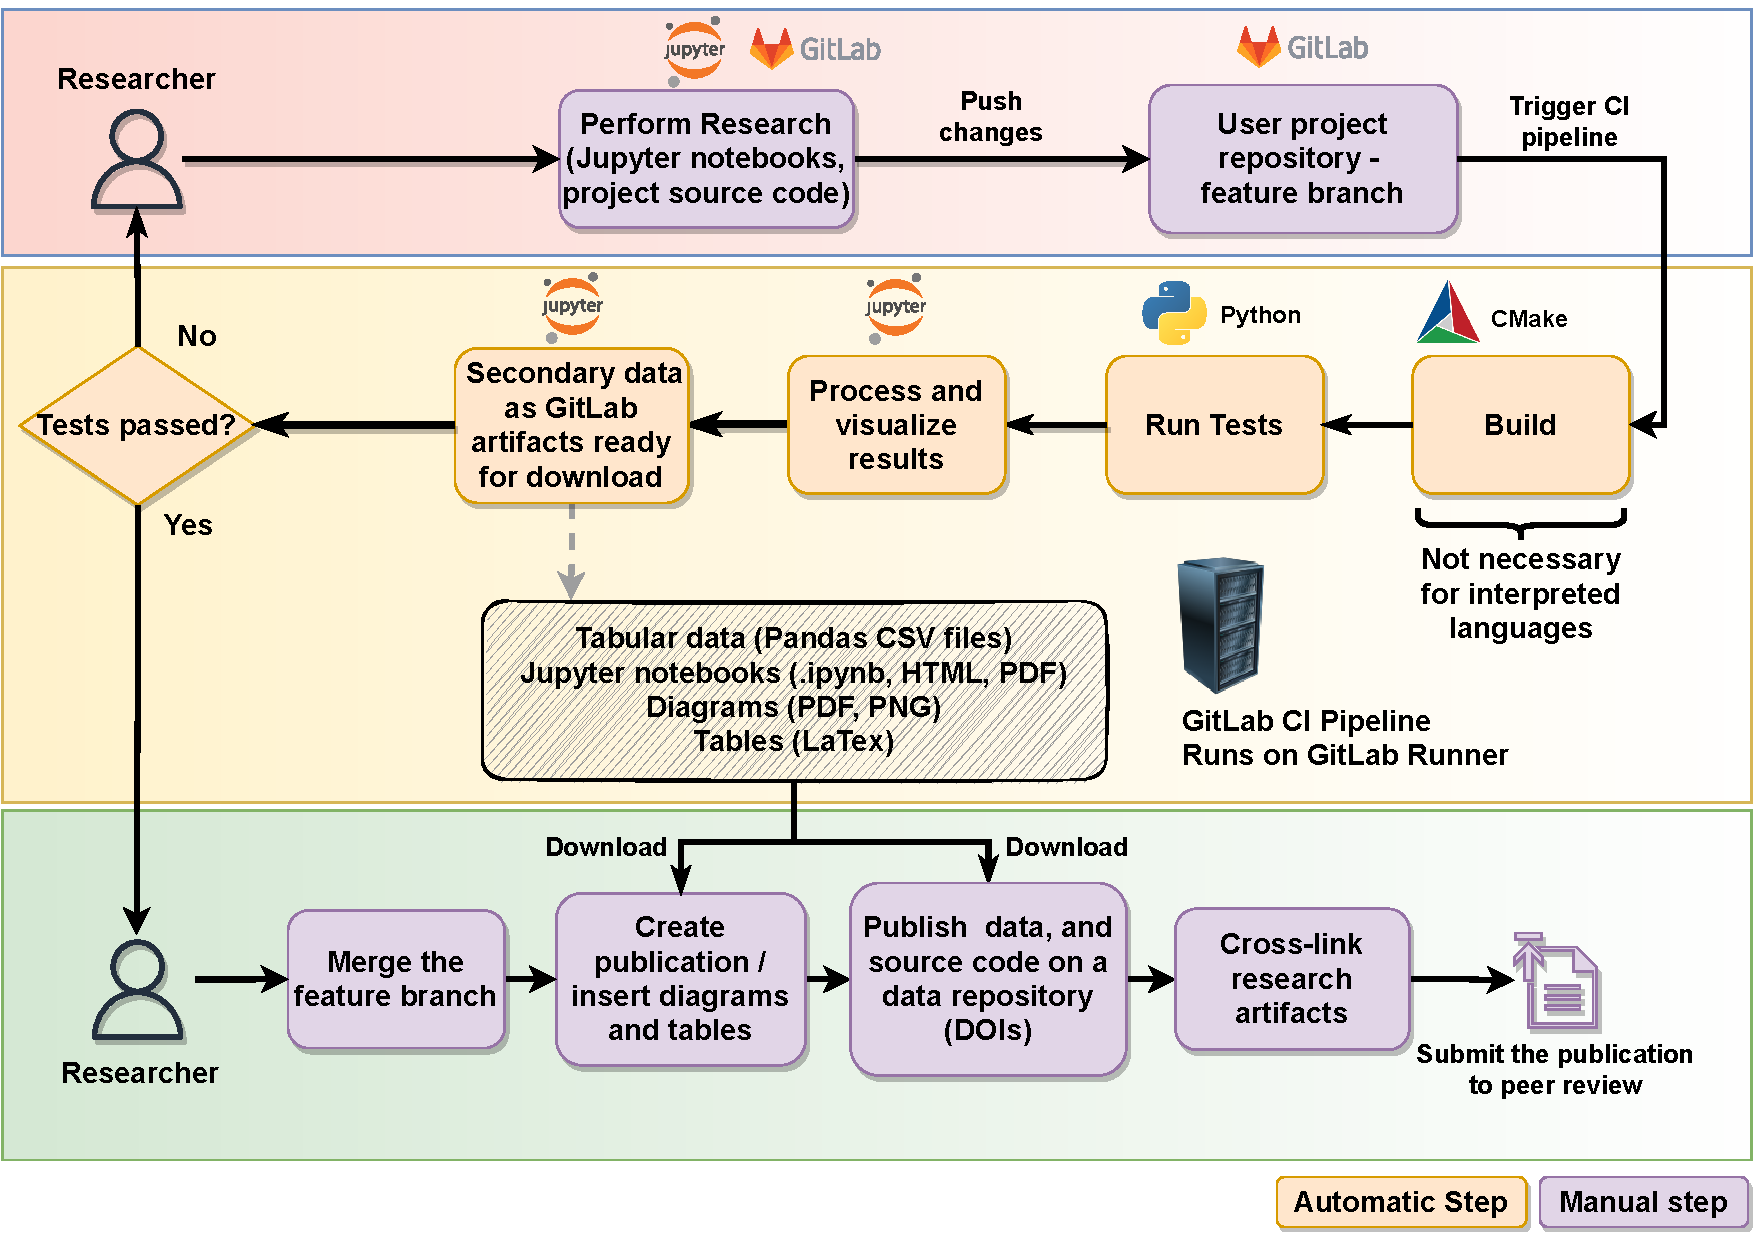
\includegraphics[scale=0.27]{figures/ZINF-CI-diagram-individual.drawio.pdf}
}
\date{HiPerCH-13 2021-09-23}

\usepackage{booktabs}
\usepackage{fontawesome}
\usepackage{epigraph}
\setlength{\epigraphwidth}{0.8\textwidth}

\usepackage{algorithm}
\usepackage{algpseudocode}
\usepackage{minted}

\hypersetup{
  colorlinks,
  citecolor=violet,
  linkcolor=red,
  urlcolor=violet
}

\usepackage{tikz}
\usepackage{tikzsymbols}
\usetikzlibrary{
    calc,
    trees,
    positioning,
    matrix,
    chains,
    scopes,
    fit,
    shapes,
    backgrounds,
    decorations.pathreplacing,%
    decorations.pathmorphing%
}
\tikzset{
    >=latex,
    % For block diagrams
    root/.style={
        fill=black!50,
        draw=black,
        thick,
        rounded corners,
        inner sep=1em,
        minimum width=2cm
    },
    child/.style={
        root,
        fill=black!50
    },
    % Nesting things
    nest/.style={
        matrix of nodes,
        nodes=chick,
        row sep=1em,
        inner sep=0pt
    },
    nestContainer/.style={
        draw=black,
        align=center,
        inner sep=1ex
    },
    chick/.style={
        draw=black,
        fill=black!50,
        rounded corners,
        inner sep=1ex,
        anchor=center
    },
    nestName/.style={
        color=black,
        draw=none,
        fill=none,
        font=\bfseries,
        inner sep=1ex
    },
    % TIKZ inline
    inline/.style={
        remember picture,
        baseline=-.5ex
    },
    inlineCode/.style={
        inline,
        rectangle,
        font={\ttfamily},
        draw=black,
        fill=black!10,
        rounded corners,
        inner sep=1ex
    }
}
\usepackage{tikzscale}


\begin{document}

\setbeamertemplate{footline}{%
    \hbox{%
    \begin{beamercolorbox}[wd=.70\paperwidth,ht=4.25ex,dp=3ex,left,leftskip=4ex]{title in head/foot}%
        \usebeamerfont{title in head/foot}\insertshorttitle{} - \insertshortauthor
    \end{beamercolorbox}%
    \begin{beamercolorbox}[wd=.20\paperwidth,ht=4.25ex,dp=3ex,center]{date in head/foot}%
        \usebeamerfont{date in head/foot}\insertshortdate{}
    \end{beamercolorbox}%
    \begin{beamercolorbox}[wd=.10\paperwidth,ht=4.25ex,dp=3ex,right,rightskip=5ex]{date in head/foot}%
        \insertframenumber{} / \inserttotalframenumber
    \end{beamercolorbox}}%
}


\maketitle

\section{Introduction}

\begin{frame}{Motivation: multiphase flow simulation methods}
    \framesubtitle{Lagrangian / Eulerian Interface Advection (LEIA) methods}

    \begin{center}
    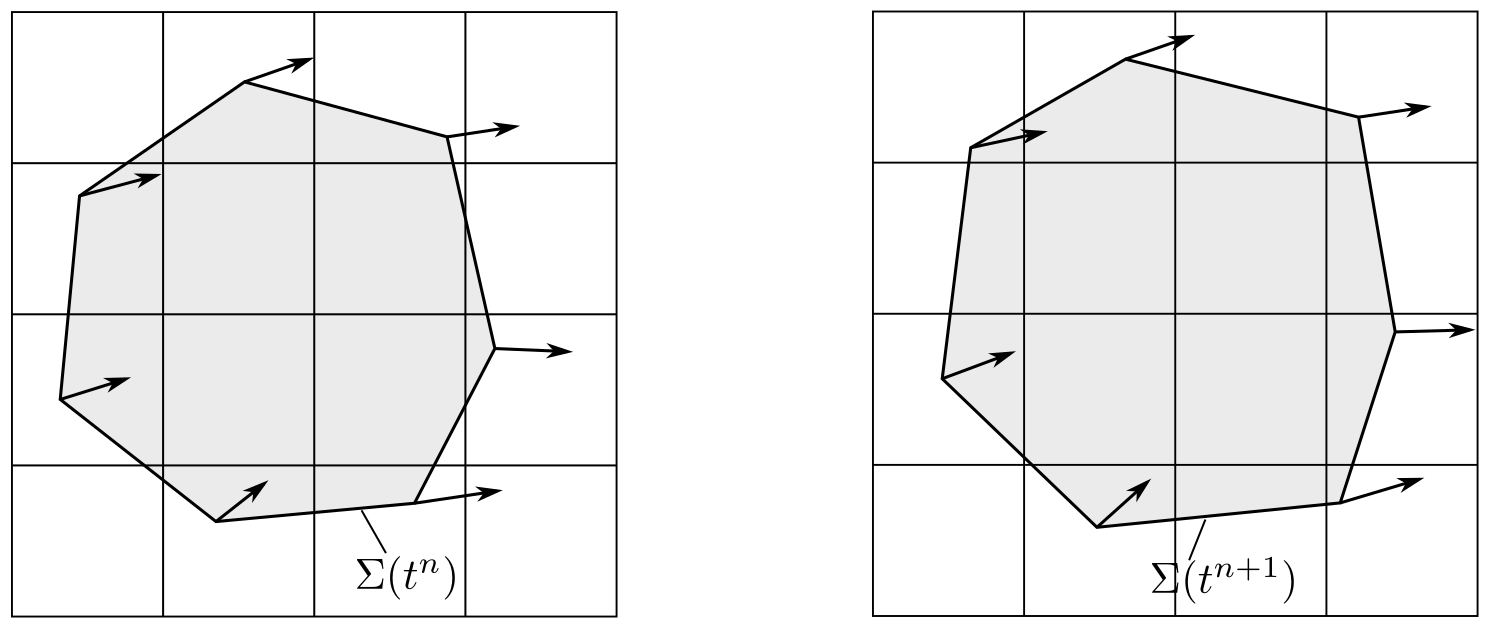
\includegraphics[width=0.7\textwidth]{figures/interface.png}
    \end{center}
    \begin{itemize}
        \item Fluids that do not mix are separated by an interface $\Sigma(t)$ (surface in 3D). 
        \item Goal: track $\Sigma(t)$ as it moves in time $t$ and changes its topology. 
    \end{itemize}

\end{frame}

\begin{frame}{Motivation: multiphase flow simulation software}
    \framesubtitle{Lagrangian / Eulerian Interface Advection (LEIA) Methods}

    \vfill
    LEIA methods
    \footnote{Marić, T., Marschall, H., \& Bothe, D. (2015). lentFoam–A hybrid Level Set/Front Tracking method on unstructured meshes. Computers \& Fluids, 113, 20-31.}\textsuperscript{,}
    \footnote{\footnotesize Tolle, T., Bothe, D., \& Marić, T. (2020). SAAMPLE: A Segregated Accuracy-driven Algorithm for Multiphase Pressure-Linked Equations. Computers \& Fluids, 200, 104450.}\textsuperscript{,}
    \footnote{Marić, T., Kothe, D. B., \& Bothe, D. (2020). Unstructured un-split geometrical Volume-of-Fluid methods–A review. Journal of Computational Physics, 420, 109695.}\textsuperscript{,}
    \footnote{\footnotesize Marić, T. (2021). Iterative Volume-of-Fluid interface positioning in general polyhedrons with Consecutive Cubic Spline interpolation. Journal of Computational Physics: X, 11, 100093.}\textsuperscript{,}
    \footnote{\footnotesize Tolle, T., Gründing, D., Bothe, D., \& Marić, T. (2021). Computing volume fractions and signed distances from triangulated surfaces immersed in unstructured meshes. arXiv preprint arXiv:2101.08511.}
    require \textbf{thorough testing}: 
    \begin{itemize}
        \item \textbf{Verification} cases: evolution of $\Sigma(t)$ and two-phase flows with exact solutions. 

        \item \textbf{Validation} with respect to experiments.  

        \item Testing \textbf{serial and parallel computational efficiency}. 
    \end{itemize}

\end{frame}

%\begin{frame}{Motivation: Level Set / Front Tracking method\footnote{\footnotesize Marić, T., Marschall, H., \& Bothe, D. (2015). lentFoam–A hybrid Level Set/Front Tracking method on unstructured meshes. Computers \& Fluids, 113, 20-31.},\footnote{\footnotesize Tolle, T., Bothe, D., \& Marić, T. (2020). SAAMPLE: A Segregated Accuracy-driven Algorithm for Multiphase Pressure-Linked Equations. Computers \& Fluids, 200, 104450.}}

    %\vfill
    %\begin{center}
        %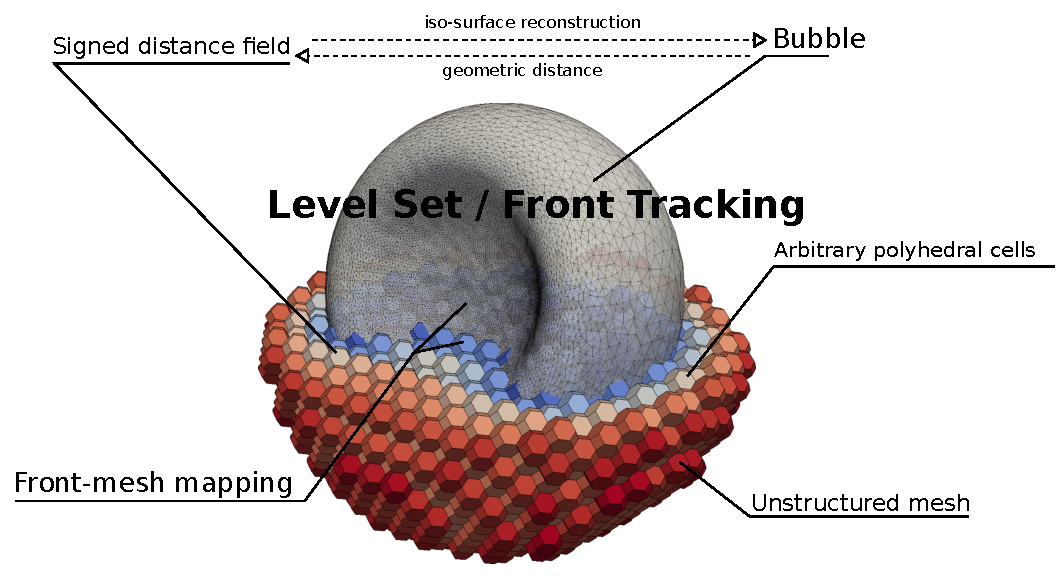
\includegraphics[width=0.5\textwidth]{figures/lent-schematic.pdf}
    %\end{center}
%\end{frame}

%\begin{frame}{Motivation: geometrical un-split Volume-of-Fluid method\footnote{Marić, T., Kothe, D. B., \& Bothe, D. (2020). Unstructured un-split geometrical Volume-of-Fluid methods–A review. Journal of Computational Physics, 420, 109695.}}

    %\vfill
    %\begin{center}
        %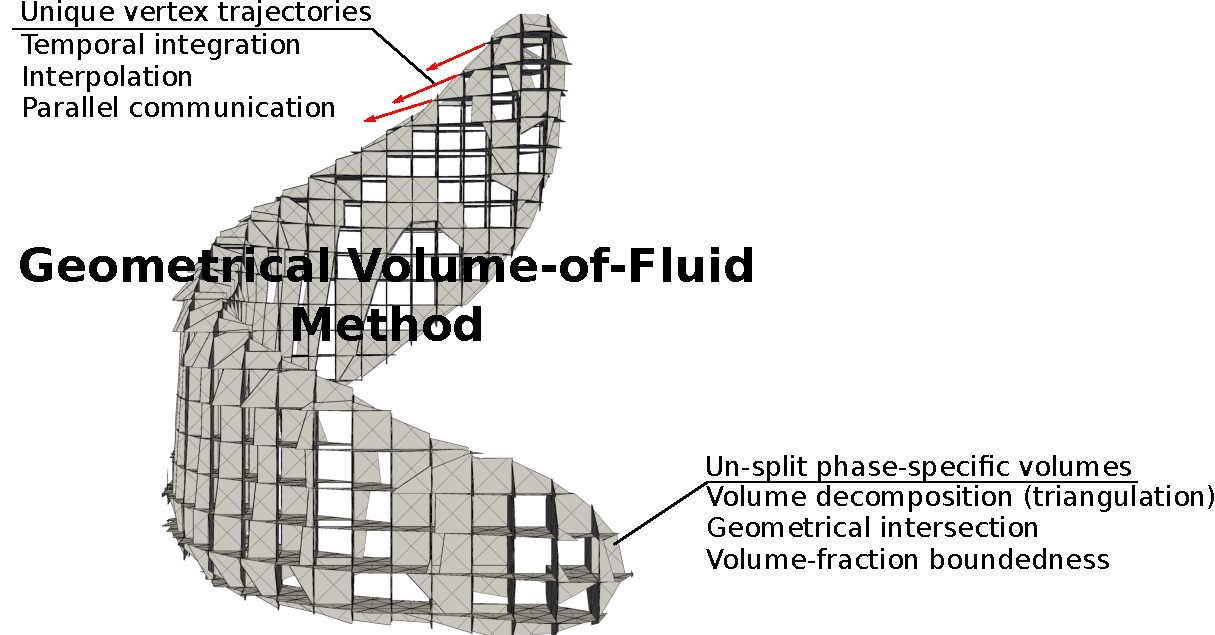
\includegraphics[width=0.6\textwidth]{figures/geovof-schematic.pdf}
    %\end{center}
%\end{frame}

\begin{frame}{Computational Science and Engineering software in\\university research groups}
	\framesubtitle{Boundary and initial conditions}
	
	\vfill
	\begin{itemize}
            \item Publish or perish \faGraduationCap\footnote{Symbol of a publish-or-perish simplification of the workflow :)} prioritizes publications over scientific software.
		\item Dedicated resources for increasing software quality are usually not available.
		\item Ph.D. students rotate every ~3-5 years, postdocs every 1-2 years. 
			\begin{itemize}
				\item Little or no overlap between successors and predecessors. 
			\end{itemize}
		\item Large-scale software design is not a necessary part of the CSE curriculum. 
			\begin{itemize}
				\item Different CSE background: (Applied) Mathematics, Mechanical Engineering, Physics, Informatics.
			\end{itemize}
		\item Real-world example: onboarding people into \href{https://www.openfoam.com/documentation/guides/latest/api/classes.html}{\beamergotobutton{OpenFOAM}} module development.
	\end{itemize}
\end{frame}

\begin{frame}{NFDI4Ing to the rescue!}
\framesubtitle{Resources for engineering research software}
    \vfill

    \begin{center}
    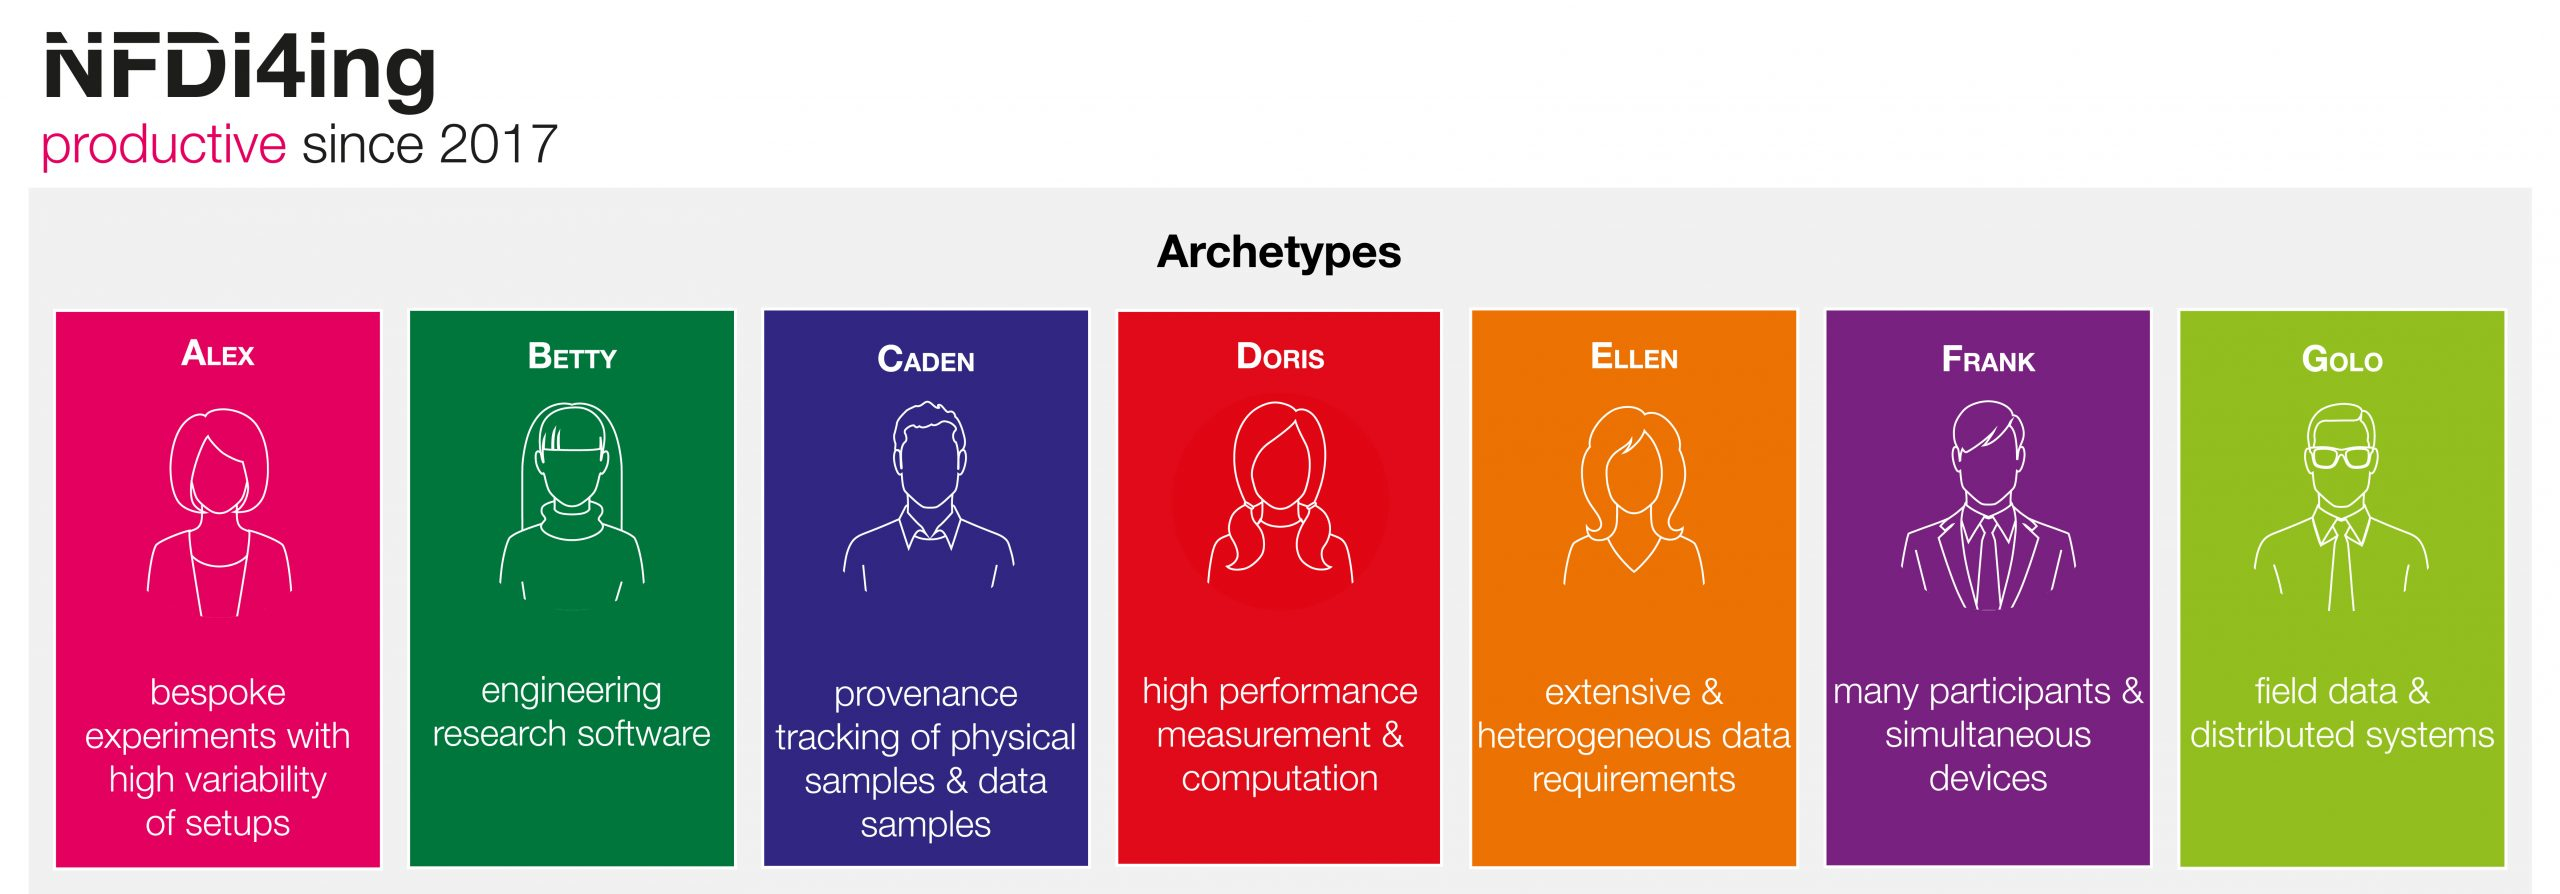
\includegraphics[width=\textwidth]{figures/nfdi4ing.jpg}
    \end{center}
    \href{https://nfdi4ing.de}{NFDI4Ing} resources. 

\end{frame}

\begin{frame}{BSSW to the rescue!}
\framesubtitle{Resources for engineering research software}
    \vfill

    \begin{center}
    
\includegraphics[width=0.6\textwidth]{figures/bssw.png}
    \end{center}
    \href{https://bssw.io}{Better Scientific Software} resources. 

\end{frame}


\begin{frame}{Computational Science and Engineering software in\\university research groups}
    \framesubtitle{The chaos scientific legacy code}
        \vfill
	
    \begin{columns}
        \begin{column}[c]{0.2\textwidth}
            \begin{center}
            
\includegraphics[width=\textwidth]{figures/betty.jpg}
            \end{center}
        \end{column}
        \begin{column}[c]{0.8\textwidth}
            Betty is a CSE researcher, working with a legacy research code.\\
            Why is Betty so (rightfully) angry? 
            \begin{itemize}
                \item Betty inherited a \textbf{research software that is only partially tested}.
                \item Betty inherited a \textbf{research software that isn't automatically tested}.
                    \begin{itemize}
                        \item Betty changes one part of the code and gets her model running, only to see 10 other things fail, after days of manually running tests. 
                    \end{itemize}
                \item Betty's software has \textbf{no documentation of the scientific workflow}. 
                    \begin{itemize}
                        \item Betty doesn't know how to use existing scripts to run simulations and analyze (reproduce) results. 
                    \end{itemize}
                \item Betty's software has \textbf{disjoint (diverging) versions} - that she can't integrate. 
                \item \textbf{Betty can't even find code versions used to generate results in the publications from her research group.} 
            \end{itemize}
        \end{column}
    \end{columns}

\end{frame}

\begin{frame}{Computational Science and Engineering software in\\university research groups}
    \framesubtitle{The chaos of developing entirely new research software}
    \vfill

    \epigraph{"Après moi, le déluge" - "After me, the flood"}{\href{https://en.wikipedia.org/wiki/Apr\%C3\%A8s_moi,_le_d\%C3\%A9luge}{Louis XV of France}}

    Research software generally does not matter, as long as papers are published (\faGraduationCap).
    
    \medskip

    \textbf{Missed opportunities}
    \begin{itemize}
        \item \emph{Finding results} made easy by cross-linking code versions, data and publications. 
        \item \emph{Faster extension / combination of existing ideas} if their respective versions are integrated. 
        \item \emph{Faster comparison of results} with previous ideas automating verification / validation. 
        \item \emph{Automatic reproducibility} of results using automated testing and version control. 
        \item \emph{Faster onboarding} with documented scientific verification and validation workflows. 
    \end{itemize}

\end{frame}

\begin{frame}{Computational Science and Engineering software in\\university research groups}
    \framesubtitle{Continuous integration and cross-linking to the rescue}
    \vfill

    \textbf{Automated testing} (verification and validation), \textbf{version control}, and \textbf{cross-linking} reports, source code and research data increase Findability, Accessibility and Reproducibility (\href{ https://www.go-fair.org/fair-principles}{FAIR}) and \textbf{speed up research.} 

    \begin{itemize}

        \item \textbf{Continuous Integration (CI) = automatic testing + version control.}

        \item CSE research requires \textbf{scientific workflows}: initialize simulations, run parameter variations, agglomerate data, visualize, and check results.  
        \item CI can be used to \textbf{automate and document scientific workflows}. 
        \item CI ensures that the \textbf{integration of new changes does not break existing functionality}.
        \item Once the changes are integrated, the publication, the source code and the data are published on pre-print and data repositories and \textbf{cross-linked} git tags and DOIs. 
    \end{itemize}

\end{frame}


%\section{Workflow overview}

\begin{frame}{A workflow for increasing the quality of scientific CSE software} 

    \vfill
    The workflow is using GitLab, specifically \href{https://git.rwth-aachen.de/}{TUGitLab}. 
    Optional steps are in round () brackets.
    \begin{enumerate}
        \item Track the issues in a Kanban board. 
            \begin{itemize}
                \item Model issues as \href{https://betterscientificsoftware.github.io/PSIP-Tools/PTCs/}{Progress Tracking Cards}\footnote{Developed by \href{https://bssw.io/}{Better Scientific Software.}}.
            \end{itemize}
        \item Use version-control with a simple branching model. 
        \item (Apply Test-Driven Development (TDD) for CSE software.)
        \item (Enable Continuous Integration with an emphasis on result visualization.) 
        \item Cross-link software, result data, and report/article when reaching a milestone.
            \begin{itemize}
                \item When submitting a publication to peer-review. 
                \item After the publication has been accepted. 
                \item When giving up on an idea. 
            \end{itemize}
        \item (Publish a Singularity image with the code and data.)
    \end{enumerate}
\end{frame}

\begin{frame}{A workflow for increasing the quality of (academic) CSE software} 
    \framesubtitle{OpenFOAM}

        \vfill

        The workflow is developed with OpenFOAM projects but it is tested with other software. 

        \vspace{1cm}

        \textbf{Disclaimer}: This offering is not approved or endorsed by OpenCFD Limited, producer and distributor of the OpenFOAM software via www.openfoam.com, and owner of the OPENFOAM®  and OpenCFD®  trade marks. 

\end{frame}

%\section{Issue tracking}

\begin{frame}{Issue tracking on GitLab Kanban boards} 
    \framesubtitle{Why use issue tracking?}
    \vfill

    Coordinating work on shared text-based information: different people editing same files.\\ 
    Tracking the status of tasks, bugs, and ideas in one place.\\
    Avoiding situations like these:
    \begin{itemize}  
        \item Why did we try that model a year ago?
        \item What was that bug in X?
        \item Meetings for discussing task status. 
            \begin{itemize}
                \item Fine for a Ph.D. student in a single project, not so fine for a postdoc with 5 projects. 
                \item Not necessary if no input is required, only the status update. 
            \end{itemize}
    \end{itemize}

\end{frame}

\begin{frame}{Issue tracking on GitLab Kanban boards} 
    \framesubtitle{Kanban board at TUGitLab}
    \vfill

    \begin{figure}
        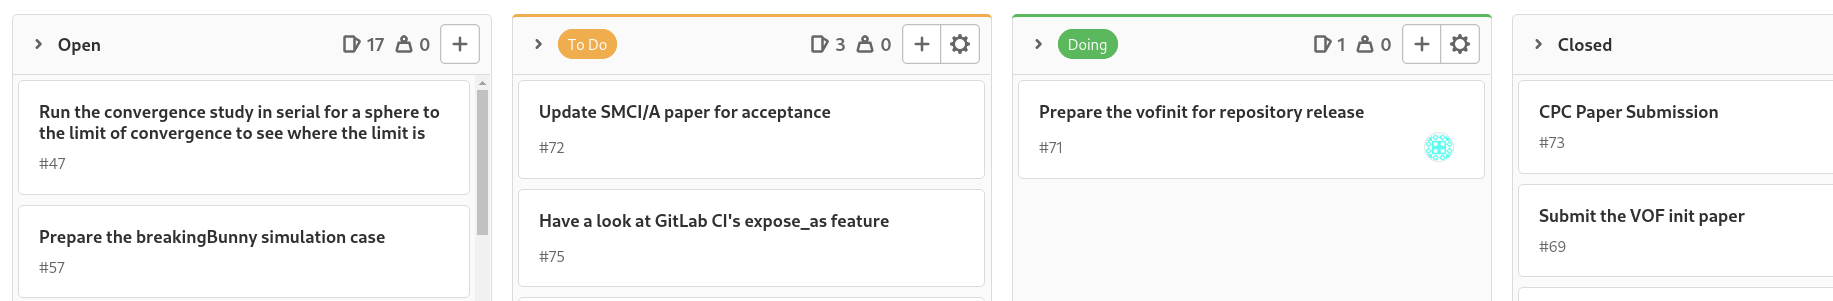
\includegraphics[width=\textwidth]{figures/kanban-board-gitlab.png}
    \end{figure}

    \begin{itemize}
        \item Create tasks and update their status.  
        \item Great for problems / bugs that can't be solved immediately. 
        \item Descriptions and comments can be done within the tasks (no searching through emails).  
    \end{itemize}

\end{frame}

\begin{frame}{Issue tracking on GitLab Kanban boards} 
    \framesubtitle{Progress Tracking Cards I}
    \vfill

    \href{}{Progress Tracking Cards}\footnote{\href{https://bssw.io/}{https://bssw.io/} Better Scientific Software} are great for teamwork.
    \begin{enumerate}  
        \item Title the task that will be solved by the team in terms of what will be achieved.
        \item Separate the task into subtasks and mention who is responsible for what. 
            \begin{itemize}
                \item Each sub-task is titled based on the achieved result.
            \end{itemize}
        \item Comment in the task, chat on Slack (Discord, ...) if more discussion is necessary, Zoom / meet if even more discussion is necessary.
    \end{enumerate}

\end{frame}

%\section{Version control}

\begin{frame}{Software engineering: version control}
    \framesubtitle{What is version control?}

    \vfill
    \begin{itemize}
        \item Management of versions of (usually) textual data, like publications and scientific codes.
        \item Nowadays version control is \textbf{essential} for scientific codes of all shapes and sizes.
        \item A basis for productive research in teams and increasing the quality of scientific software\footnote{Maric, Tomislav, Lehr, Jan-Patrick, Papagiannidis, Ioannis, Lambie, Benjamin, Bothe, Dieter, \& Bischof, Christian. (2021, April). A Workflow for Increasing the Quality of Scientific Software (Version 1.0). Zenodo. \url{http://doi.org/10.5281/zenodo.4668439}}. 
    \end{itemize}


\end{frame}

\begin{frame}{Software engineering: version control}
    \framesubtitle{Why use version control?}

    \vfill
    Why use version control in scientific codes?  
    \begin{itemize}
        \item The ability to work with others (colleagues or students) on your research project. 
            \begin{itemize}
                \item Work together faster.
                \item Re-use an interpolation method of a colleague in the group.
            \end{itemize}
        \item The ability to trivially try out new ideas and switch back if they don't work.
            \begin{itemize}
                \item Speeds up research!
            \end{itemize}
        \item The ability to easily recover versions of your project in the same folder. 
            \begin{itemize}
                \item Recovering a specific version in a predecessor project code.
            \end{itemize}
        \item The ability to understand the motivation behind changes via comments. 
            \begin{itemize}
                \item Crucial for continuing existing research projects.
            \end{itemize}
        \item The ability to increase the reproducibility of scientific results. 
            \begin{itemize}
                \item Basis for cross-linking of data, source code and publications / reports.  
            \end{itemize}
    \end{itemize}

\end{frame}

\begin{frame}{Software engineering: version control}
    \framesubtitle{Git version control system (VCS)}

    \vfill
    \begin{center}
        
\includegraphics[width=0.3\textwidth]{figures/Git-Logo-2Color.eps}
    \end{center}

    \begin{itemize}
        \item An effective and easy to use software with a set of commands for version control. 
    \end{itemize}

\end{frame}

\begin{frame}{Software engineering: version control}
    \framesubtitle{Git basics on a single slide}

    \vfill
    \begin{itemize}
        \item The code/text folder is called a \textbf{repository}.
        \item An online folder shared with the team is the \textbf{remote repository} (short: remote).
        \item Create a new version: \textbf{checkout} a new \textbf{branch}.  
        \item Integrate with another version: \textbf{merge} with a \textbf{branch}.
        \item Add changes in a branch: \textbf{add} changes.
        \item Integrate changes into a branch: \textbf{commit} changes.
        \item Share changes with others: \textbf{push} to \textbf{upstream repository}. 
        \item Get latest changes: \textbf{pull} from the \textbf{upstream repository}.
    \end{itemize}

\end{frame}

\begin{frame}{Software engineering: version control}
    \framesubtitle{Git basics: resources}
    \vfill

    Learn basic git \emph{concepts}, they are the same everywhere.  
    \begin{itemize}
        \item \href{https://www.youtube.com/watch?v=USjZcfj8yxE}{Git in 15 minutes} 
        \item \href{https://de.mathworks.com/help/matlab/source-control.html}{Git within Matlab}
        \item \href{https://www.atlassian.com/git/tutorials/comparing-workflows/feature-branch-workflow}{Feature branch workflow}
        \item \href{https://www.youtube.com/watch?v=Jt4Z1vwtXT0}{GitLab for beginners}
    \end{itemize}

\end{frame}

\begin{frame}{Software engineering}
    \framesubtitle{Decentralized version control}

    \vfill
    \centering
    \resizebox{.35\textwidth}{!}{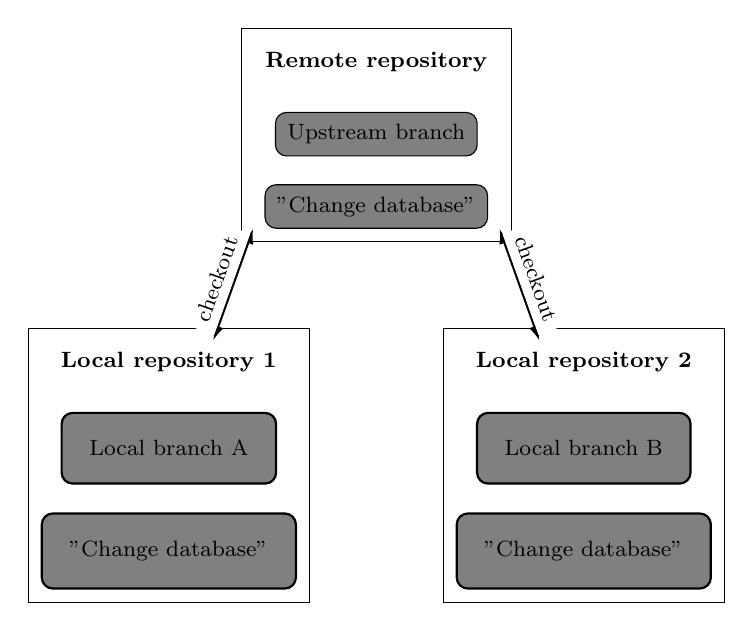
\begin{tikzpicture}[scale=0.5]

    \matrix[nest] (server) {
        |[nestName]| \footnotesize Remote repository \\
        | (serverDB) | \footnotesize Upstream branch \\
        | (serverDB) | \footnotesize "Change database" \\
    };
    \matrix[nest, left=of server.south, matrix anchor=north east,yshift=-4em] (child1) {
        |[nestName]| \footnotesize Local repository 1 \\
        |[child] (version1) | \footnotesize Local branch A \\
        |[child] (version1) | \footnotesize "Change database"\\
    };
    \matrix[nest, right=of server.south, matrix anchor=north west,yshift=-4em] (child2) {
        |[nestName]| \footnotesize Local repository 2 \\
        |[child] (version2) | \footnotesize Local branch B \\
        |[child] (version1) | \footnotesize "Change database" \\
    };
    \node[nestContainer, fit=(server)] {};
    \node[nestContainer, fit=(child1)] {};
    \node[nestContainer, fit=(child2)] {};

    \draw[<->,thick] (child1) -- node[midway,above,sloped,fill=white] {\footnotesize checkout} (server.south west);
    \draw[<->,thick] (child2) -- node[midway,above,sloped,fill=white] {\footnotesize checkout} (server.south east);

\end{tikzpicture}

\unskip}

    \begin{itemize}
        \item \textbf{Although git tracks only changes, every repository is still a complete copy of the project.}
        \item Offline work is supported!  
    \end{itemize}

\end{frame}

\begin{frame}{Software engineering: version control}
    \framesubtitle{Version control "enforces" modularity}

    \vfill

    Git conflicts 
    \begin{itemize}
        \item A file is changed differently on two branches and a merge is needed.
        \item Two team members edit the same file at once. 
    \end{itemize}

    \textbf{Modularity reduces conflicts and speeds up teamwork}
    \begin{itemize}
        \item Book chapters as separate files vs. book chapters as folders and sections as separate files.
    \end{itemize}

\end{frame}

\begin{frame}{Software engineering: version control}
    \framesubtitle{Modularity via Separation of Concerns and Single Responsibility}

	\vfill
	\begin{itemize}

            \item University research teams (like our LEIA lecture team!) are generally small (2 - 5 members).
            \item \href{https://en.wikipedia.org/wiki/Separation_of_concerns}{\beamergotobutton{Separation of Concerns (SC)}} and \href{https://en.wikipedia.org/wiki/Single-responsibility_principle}{\beamergotobutton{Single Responsibility Principle (SRP)}} significantly simplify the branching model. 

            \item \textbf{Separation of Concerns}: code is organized in non-overlapping layers and sections. 

            \item \textbf{Single Responsibility}: functions or classes perform single clear tasks.

            \item SC and SRP can be applied to any software.
            \item Dogmatism should be avoided: single responsibility vs less responsibilities. 
        \end{itemize}


\end{frame}


\begin{frame}{Simple version-control branching model} 
    \framesubtitle{Separation of Concerns and Single Responsibility}

	\vfill
	\begin{itemize}

            \item University research teams \emph{working on the same project} are generally small (2 - 5 members).
            \item \href{https://en.wikipedia.org/wiki/Separation_of_concerns}{\beamergotobutton{Separation of Concerns (SC)}} and \href{https://en.wikipedia.org/wiki/Single-responsibility_principle}{\beamergotobutton{Single Responsibility Principle (SRP)}} significantly simplify the branching model. 

            \item \textbf{Separation of Concerns}: code is organized in non-overlapping layers and sections. 

            \item \textbf{Single Responsibility}: functions or classes perform single clear tasks.

            \item SC and SRP can be applied to any software.
            \item Dogmatism should be avoided: single responsibility vs less responsibilities. 
            \item OpenFOAM already uses object-oriented and generic software design patterns.  

        \end{itemize}
\end{frame}

\begin{frame}{Simple version-control branching model} 
    \framesubtitle{Change integration}

        \vfill

        \textbf{Maintainers (postdocs, experienced Ph.D.\ students) manage the integration.} 

	\begin{itemize}
            \item Keep the branching model as simple as possible.  
            \item Main and development branches are protected and managed by Maintainers. 
            \item Maintainers are responsible for git tags and cleanup: 
            \begin{itemize}
                    \item \textbf{Main}: integrations from \emph{accepted publications} and \emph{development branch}. 
                    \item \textbf{Development}: integration of \emph{(CI)-tested improvements}. 
                    \item \textbf{Feature}: SRP reduces git-conflicts with researchers working on different files.
            \end{itemize}
            \item Complex branching workflow $\Rightarrow$ complications with onboarding new members.
	\end{itemize}

\end{frame}

%\section{Test Driven Development}

\begin{frame}{(Test Driven Development)} 
    \framesubtitle{Program CSE tests first}
        \vfill

        TDD\footnote{Freeman, Steve, and Nat Pryce. Growing object-oriented software, guided by tests. Pearson Education, 2009.} for CSE
        \begin{itemize}
            \item Define verification and validation tests at the start.
            \item Focus placed the final result: interpolation, integration, discretization, PDE solution, physics. 
            \item Top-down, instead of bottom-up test coverage.
            \item Don't go overboard with unit-tests \faGraduationCap: extend unit-tests when debugging a failing CSE test.  
            \item Focus kept on tests with real-world (publication) input. 
        \end{itemize}

\end{frame}

\begin{frame}{(Test Driven Development)} 
    \framesubtitle{Verification and validation tests define the Application Programming Interface}
        \vfill

    \begin{itemize}
        \item \textbf{New code}: it is easier to program the API you wish for, if you are its first user. 
            \begin{itemize}
                \item Make the class interface easy to use correctly and difficult to use incorrectly\footnote{Scott Meyers. 2014. Effective Modern C++: 42 Specific Ways to Improve Your Use of C++11 and C++14 (1st. ed.). O'Reilly Media, Inc.}.
                \item Reduce number of function arguments, single responsibility, clear naming, ... 
            \end{itemize}
        \item \textbf{Legacy code}: extend existing API without modification. 
            \begin{itemize}
                \item OpenFOAM: understanding class hierarchies, \textit{finding a base class with Runtime Type Selection and a virtual function to overload.}
            \end{itemize}
        \item \textbf{The test application is the solver application with a different input.}
            \begin{itemize}
                \item If possible, testing and solution is done by the same code.  
                \item This prevents code duplication. 
                \item Data output and additional checks can be disabled by (compile-time) options.
            \end{itemize}
    \end{itemize}

\end{frame}


\begin{frame}{Test Driven Development} 
    \framesubtitle{Jupyter notebooks}

    \vfill
    Jupyter notebooks\footnote{\href{https://jupyter.org/}{https://jupyter.org/}}
    \begin{itemize}
        \item \textbf{Documentation}: geometry, initial and boundary conditions, error norms, comparison data.
        \item \textbf{Processing}: verification errors (conservation, convergence, stability), validation errors. 
        \item \textbf{Result analysis}: very straightforward, interactive, remote.
    \end{itemize}
\end{frame}

\begin{frame}{Test Driven Development} 
    \framesubtitle{(Parameter tests)}
    
    \vfill
    \begin{center}
            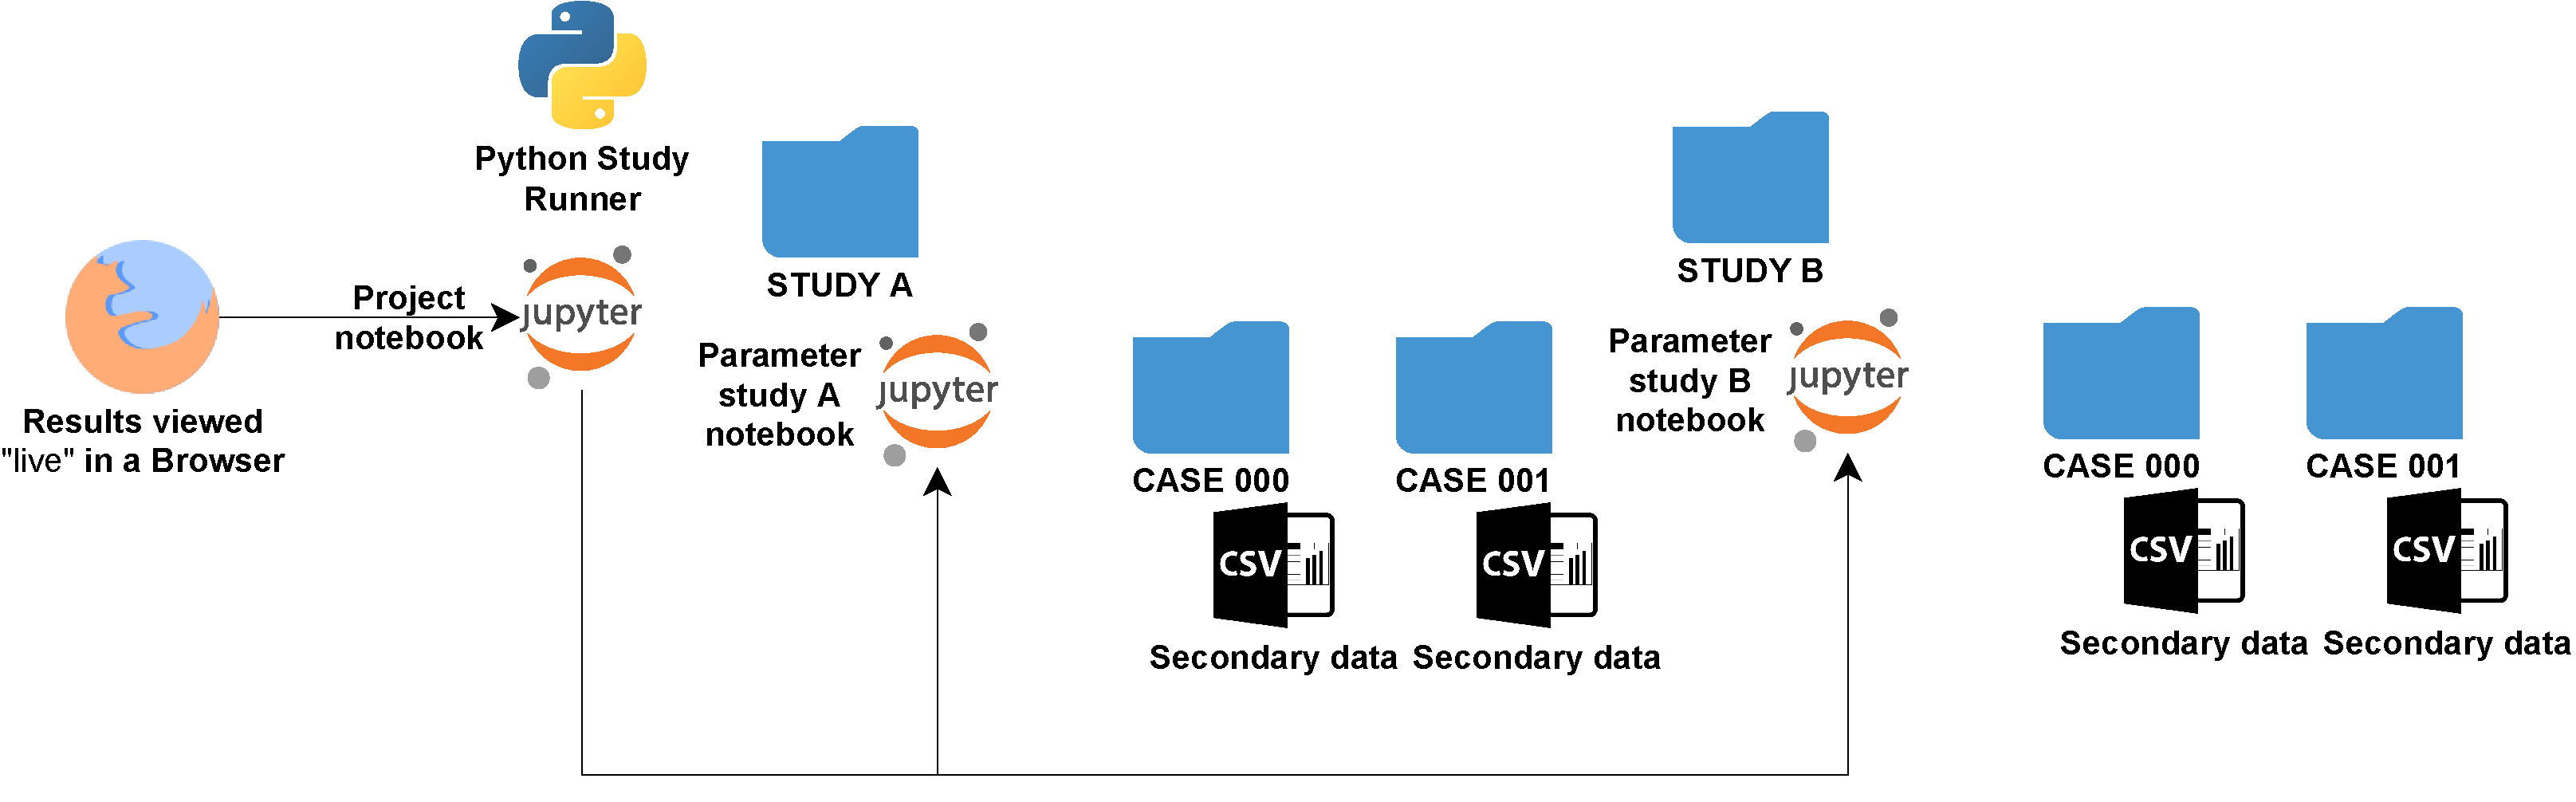
\includegraphics[width=0.9\textwidth]{figures/Cluster-Parameter-Study-Organization.pdf}
    \end{center}
\end{frame}

\begin{frame}{Test Driven Development} 
    \framesubtitle{Parameter tests: primary data (simulation results) organization}

    \begin{itemize}
        \item The quality of CSE software is measured using verification and validation data. 
        \item Effective comparison with others (previous versions) hinges on data organization.
    \end{itemize}
    
    \vfill
    \begin{itemize}
        \item \textbf{Legacy code}: 
            \begin{itemize}
                \item use the existing folder structure and parameterization tools \faGraduationCap,
                \item The mapping (case000) $\to$ (parameter vector) must be stored (YAML, ...)
            \end{itemize}
        \item \textbf{New code}: 
            \begin{enumerate}
                \item Simple folder and file structure \faGraduationCap
                \item HDF5\footnote{\url{https://www.hdfgroup.org/solutions/hdf5}} or other open data format.
                \item Alternative to HDF5: \textbf{ExDir}\footnote{Dragly, Svenn-Arne, et al. "Experimental Directory Structure (Exdir): An alternative to HDF5 without introducing a new file format." Frontiers in neuroinformatics 12 (2018): 16.} 
            \end{enumerate}
    \end{itemize}

\end{frame}


\begin{frame}{Test Driven Development} 
    \framesubtitle{Parameter tests: secondary data (tables and diagrams) organization}

    \href{https://pandas.pydata.org/}{pandas.MultiIndex} CSV with metadata for secondary data
    \begin{itemize}
        \item \texttt{pandas.MultiIndex} saved in "metadata columns". 
        \item \textcolor{red}{\textbf{Metadata is repeated}}: not an issue for the small secondary data! 
        \item Metadata in columns $\to$ \texttt{pandas.MultiIndex} $\to$ strongly simplified data analysis. 
        \item \textbf{Direct readable export of tables to LaTex!}
    \end{itemize}

    \footnotesize

    \begin{tabular}{llllll}
        \toprule
        {} &         H &     L\_INF &  O(L\_INF) &  EPSILON\_R\_EXACT\_MAX &  O(EPSILON\_R\_EXACT\_MAX)  \\ 
        VELOCITY\_MODEL &           &           &           &                      &                        \\ 
        \midrule
        \textcolor{red}{\textbf{SHEAR\_2D}}       &  0.125000 &  0.032961 &  1.833407 &             0.032961 &                1.833407 \\ 
        \textcolor{red}{\textbf{SHEAR\_2D}}       &  0.062500 &  0.009249 &  1.955529 &             0.009249 &                1.955529 \\ 
        \textcolor{red}{\textbf{SHEAR\_2D}}       &  0.031250 &  0.002385 &  1.988745 &             0.002385 &                1.988745 \\ 
        \textcolor{red}{\textbf{SHEAR\_2D}}       &  0.015625 &  0.000601 &  1.997178 &             0.000601 &                1.997178 \\ 
        \textcolor{red}{\textbf{SHEAR\_2D}}       &  0.007813 &  0.000150 &  1.999294 &             0.000150 &                1.999294 \\ 
        \textcolor{red}{\textbf{SHEAR\_2D}}       &  0.003906 &  0.000038 &  1.999294 &             0.000038 &                1.999294 \\ 
        \bottomrule
    \end{tabular}

\end{frame}

%\section{Cross-linking research data}

\begin{frame}{Cross-linking data, source code and reports/publications} 
	\framesubtitle{Schematic diagram}
	
	\begin{center}
		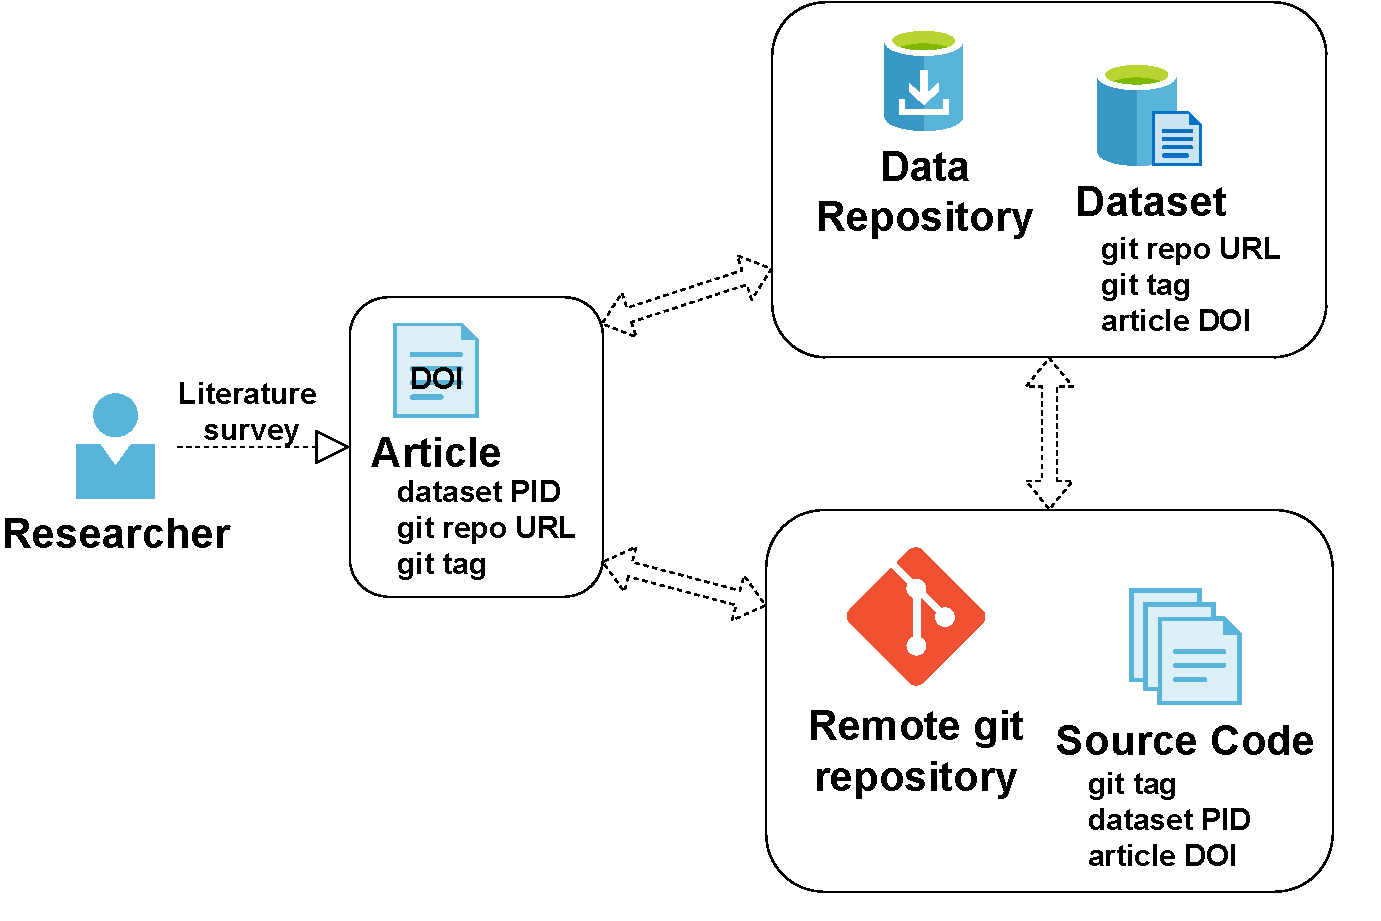
\includegraphics[width=0.67\textwidth]{figures/cross-linking.pdf}
	\end{center}

\end{frame}

\begin{frame}{(Cross-linking data, source code and reports/publications)} 
    \framesubtitle{Singularity} 
        
    \vfill
    \begin{itemize}
        \item Whence the Singularity Image\footnote{https://sylabs.io/docs/}?
            \begin{itemize}
                \item More intuitive than Docker: \textbf{Singularity handles images as files.} 
                \item Built for HPC from the start. 
                \item Doesn't require root rights. 
                \item Results as \emph{actual files}, not "data in spinning containers". 
                \item Maps user folder to the container: result data remains on the host. 
            \end{itemize}
        \item Why not replace Docker with Singularity within GitLab CI? 
            \begin{itemize}
                \item We're learning how to do this using \href{https://docs.gitlab.com/runner/executors/custom.html}{GitLab custom executors}.
                \item Does the workflow still survive publish-or-perish \faGraduationCap test?
            \end{itemize}
        \item Why a source-code snapshot on-top of the image and the repository? 
            \begin{itemize}
                \item Repositories get migrated, deleted, and some researchers still fear images. 
                \item Quick and direct access to source code from the publication. 
            \end{itemize}
    \end{itemize}

\end{frame}

\begin{frame}{(Cross-linking data, source code and reports/publications)} 
    \framesubtitle{Singularity simplifies reproducibility}

    \begin{itemize}
        \item The source code and the data stored in the image can be quickly reproduced.
        \item Article reviewers can clone, build, run and visualize easily. 
    \end{itemize}

    \href{https://git.rwth-aachen.de/leia/geophase/-/blob/JCOMP-D-19-01329R2/geophase.def}{Example: Singularity Image from an active review}
    \begin{itemize}
        \item Clone the code repository from the image: \\ \texttt{geophase-JCOMP-D-19-01329R2.sif clone geophase}
        \item Build: \\ \texttt{geophase-JCOMP-D-19-01329R2.sif build geophase build}
        \item Run tests: \\ \texttt{geophase-JCOMP-D-19-01329R2.sif run-tests geophase build}
        \item Open the jupyter notebook: \\ \texttt{geophase-JCOMP-D-19-01329R2.sif jupyter-notebook geophase}
    \end{itemize}

\end{frame}

\section{Continuous Integration overview}

\begin{frame}{Continuous Integration of Scientific Software}
    \framesubtitle{Research Software Workflow I} 
    \vfill

    \begin{columns}
        \begin{column}[c]{0.5\textwidth}
            \begin{figure}
                \centering
                
\includegraphics[width=\columnwidth]{figures/workflow-overview.png}
            \end{figure}
        \end{column}
        \begin{column}[c]{0.5\textwidth}
        \begin{algorithmic}
            \While{Results are unsatisfactory}
                \State Work on algorithms.
                \State (Compile the code.) 
                \For{All studies}
                    \State Prepare the study. 
                    \State Run the study. 
                    \State Analyze results. 
                    \State Move results to a report. 
                \EndFor
                \State Compare old and new results. 
            \EndWhile
        \end{algorithmic}
        \end{column}
    \end{columns}

\end{frame}

\begin{frame}{Continuous Integration of Scientific Software}
    \framesubtitle{Research Software Workflow II} 
    \vfill

    \begin{columns}
        \begin{column}[c]{0.5\textwidth}
            \begin{figure}
                \centering
                
\includegraphics[width=\columnwidth]{figures/workflow-overview.png}
            \end{figure}
        \end{column}
        \begin{column}[c]{0.5\textwidth}
            Issues...
            \begin{itemize}
                \item Starting studies takes time. 
                \item Analyzing results takes time. 
                \item Often the results are not checked "live" as the study runs - \textbf{waste of research time and CPUh}. 
                \item \textbf{Only the researcher knows the details} behind the initialization, running and post-processing scripts - \textbf{when this person leaves, with her/him leaves reproducibility.} 
                \item A researcher may forget to run a study and believe all tests have passed.
            \end{itemize}
        \end{column}
    \end{columns}


\end{frame}


\begin{frame}{Continuous Integration of Scientific Software}
    \framesubtitle{Automating the research workflow I} 
    \vfill

    \only<1>{
        \begin{columns}
            \begin{column}[c]{0.5\textwidth}
                \begin{figure}
                    \centering
                    
\includegraphics[width=\columnwidth]{figures/workflow-overview.png}
                \end{figure}
            \end{column}
            \begin{column}[c]{0.5\textwidth}
            %\footnotesize
            \begin{algorithmic}
                \While{Results are unsatisfactory}
                    \State Work on algorithms.
                    \State (Compile the code.) 
                    \For{All studies}
                        \State Prepare the study.
                        \State Run the study.
                        \State Analyze results. 
                        \State Move results to a report. 
                    \EndFor
                    \State Compare old and new results. 
                \EndWhile
            \end{algorithmic}
            \end{column}
        \end{columns}
    }
    \only<2>{
        \begin{columns}
            \begin{column}[c]{0.5\textwidth}
                \begin{figure}
                    \centering
                    
\includegraphics[width=\columnwidth]{figures/workflow-overview.png}
                \end{figure}
            \end{column}
            \begin{column}[c]{0.5\textwidth}
            \begin{algorithmic}
                \While{Results are unsatisfactory}
                    \State Work on algorithms.
                    \State (Compile the code.) 
                    \State Run initialization scripts (jobs).
                    \State Run simulation scripts (jobs). 
                    \State (Run postprocessing scripts (jobs)). 
                    \State Visualize results live in Jupyter notebooks. 
                \EndWhile
            \end{algorithmic}
            \end{column}
        \end{columns}
    }

\end{frame}


\begin{frame}{Continuous Integration of Scientific Software}
    \framesubtitle{Automating the research workflow II} 
    \vfill

     Manual steps of the research workflow,   
     \medskip
        \begin{algorithmic}
            \State (Compile the code.) 
            \For{All studies}
                \State Prepare the study.
                \State Run the study.
                \State Analyze results. 
                \State Move results to a report. 
            \EndFor
            \State Compare old and new results. 
        \end{algorithmic}
    \medskip
    are now automated using scripts \textbf{that do not require additional knowledge / input (metadata).} \\

\end{frame}

\begin{frame}{Continuous Integration of Scientific Software}
    \framesubtitle{Automating the research workflow III} 
    \vfill

        \begin{columns}
            \begin{column}[c]{0.5\textwidth}
                \begin{figure}
                    \centering
                    
\includegraphics[width=\columnwidth]{figures/workflow-overview.png}
                \end{figure}
            \end{column}
            \begin{column}[c]{0.5\textwidth}
                \begin{enumerate} 
                    \item The \textbf{new} results are satisfactory. 
                    \item Similar automated workflows are executed for existing tests. 
                    \item All results are checked. 
                    \item The milestone has been reached, the version can be integrated.
                \end{enumerate}
                Works well manually when there aren't many previous verification/validation tests and their analysis is relatively simple.\\
                \textbf{Are we sure we ran all the tests and everything was OK?}
                
            \end{column}
        \end{columns}
\end{frame}

\begin{frame}{Continuous Integration of Scientific Software}
    \framesubtitle{Automating the research workflow IV} 
    \vfill

        \begin{columns}
            \begin{column}[c]{0.5\textwidth}
                \begin{figure}
                    \centering
                    
\includegraphics[width=\columnwidth]{figures/workflow-overview.png}
                \end{figure}
            \end{column}
            \begin{column}[c]{0.5\textwidth}
                \begin{itemize}
                    \item Manual examination of all previous tests is prone to error - even if V\&V scripts do not require metadata. 
                    \item Manual examination is not sustainable - students are leaving...
                    \item Tests that are relevant for the research software can are added to \textbf{Continuous Integration (CI)}.  
                    \begin{itemize}
                        \item Changes are pushed to the upstream version control repository.  
                        \item The remote repository starts the so-called \textbf{CI} test pipeline (a sequence of tests). 
                        \item Tests are automatically run, processed and visualized. 
                    \end{itemize}
                \end{itemize}
            \end{column}
        \end{columns}
\end{frame}

\begin{frame}{(Continuous) Integration of scientific software} 
	\framesubtitle{Schematic diagram for the team workflow}
        \vfill

        \centering

        \begin{columns}
            \begin{column}[c]{0.55\textwidth}
                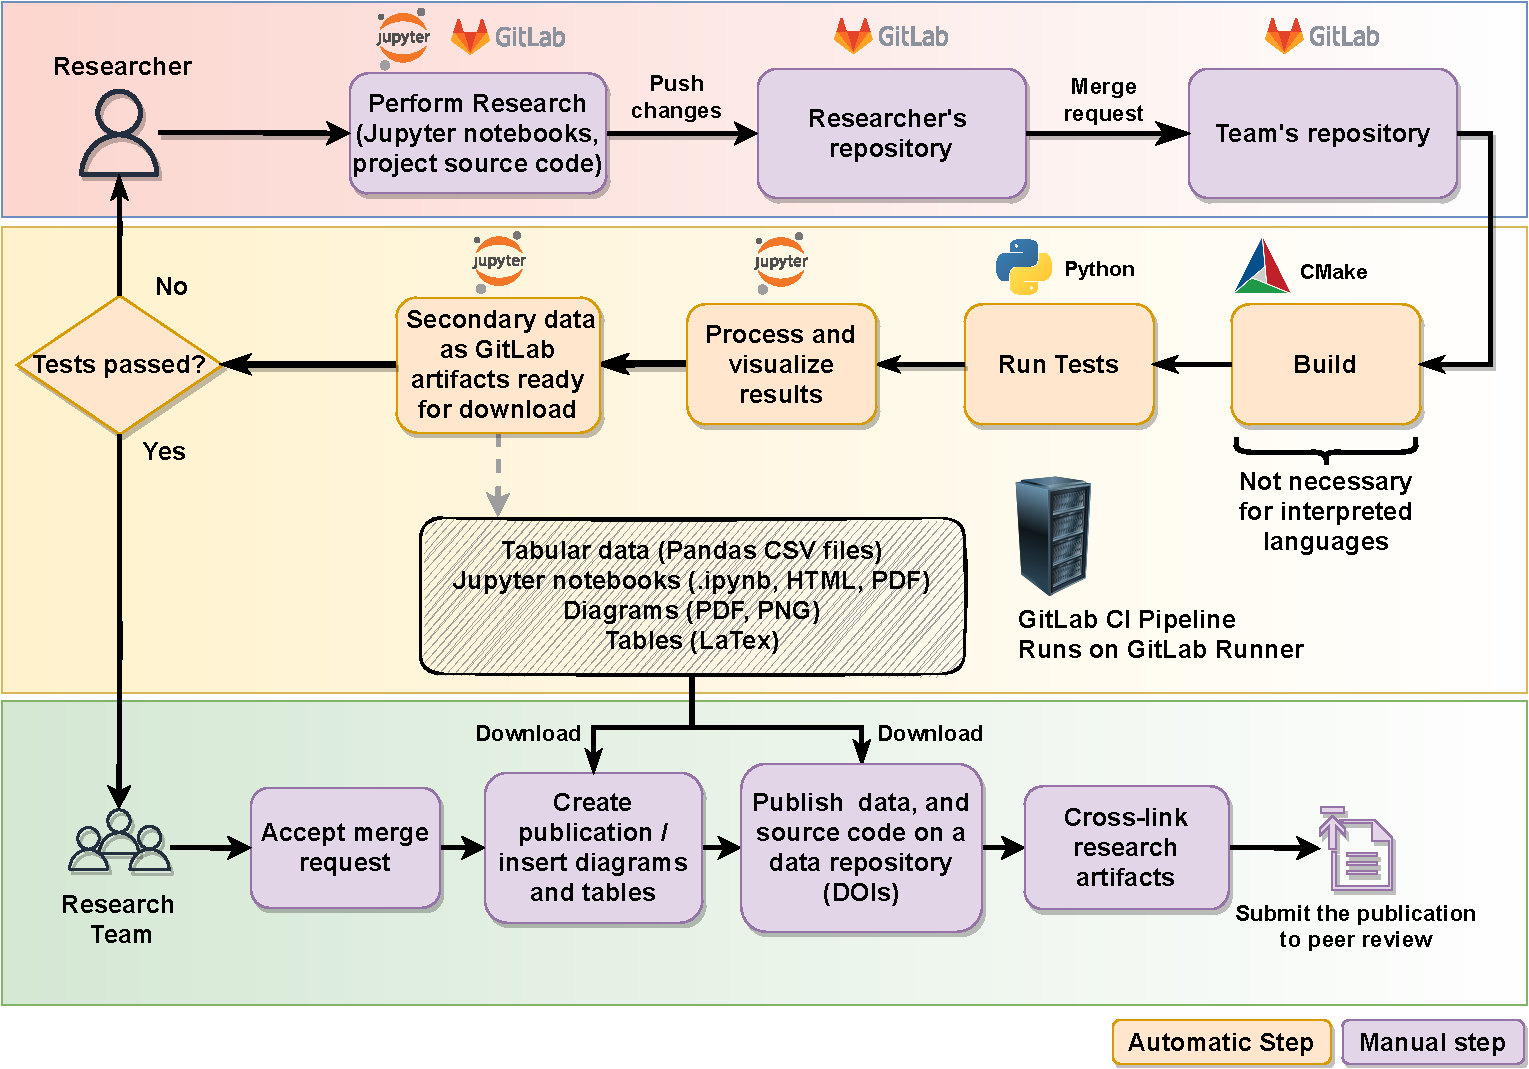
\includegraphics[width=\columnwidth]{figures/ZINF-CI-diagram.pdf}
            \end{column}
            \begin{column}[c]{0.20\textwidth}
                Working in a team.
            \end{column}
        \end{columns}
\end{frame}

\begin{frame}{(Continuous) Integration of scientific software} 
	\framesubtitle{Schematic diagram for the individual workflow}
        \vfill

        \centering

        \begin{columns}
            \begin{column}[c]{0.55\textwidth}
                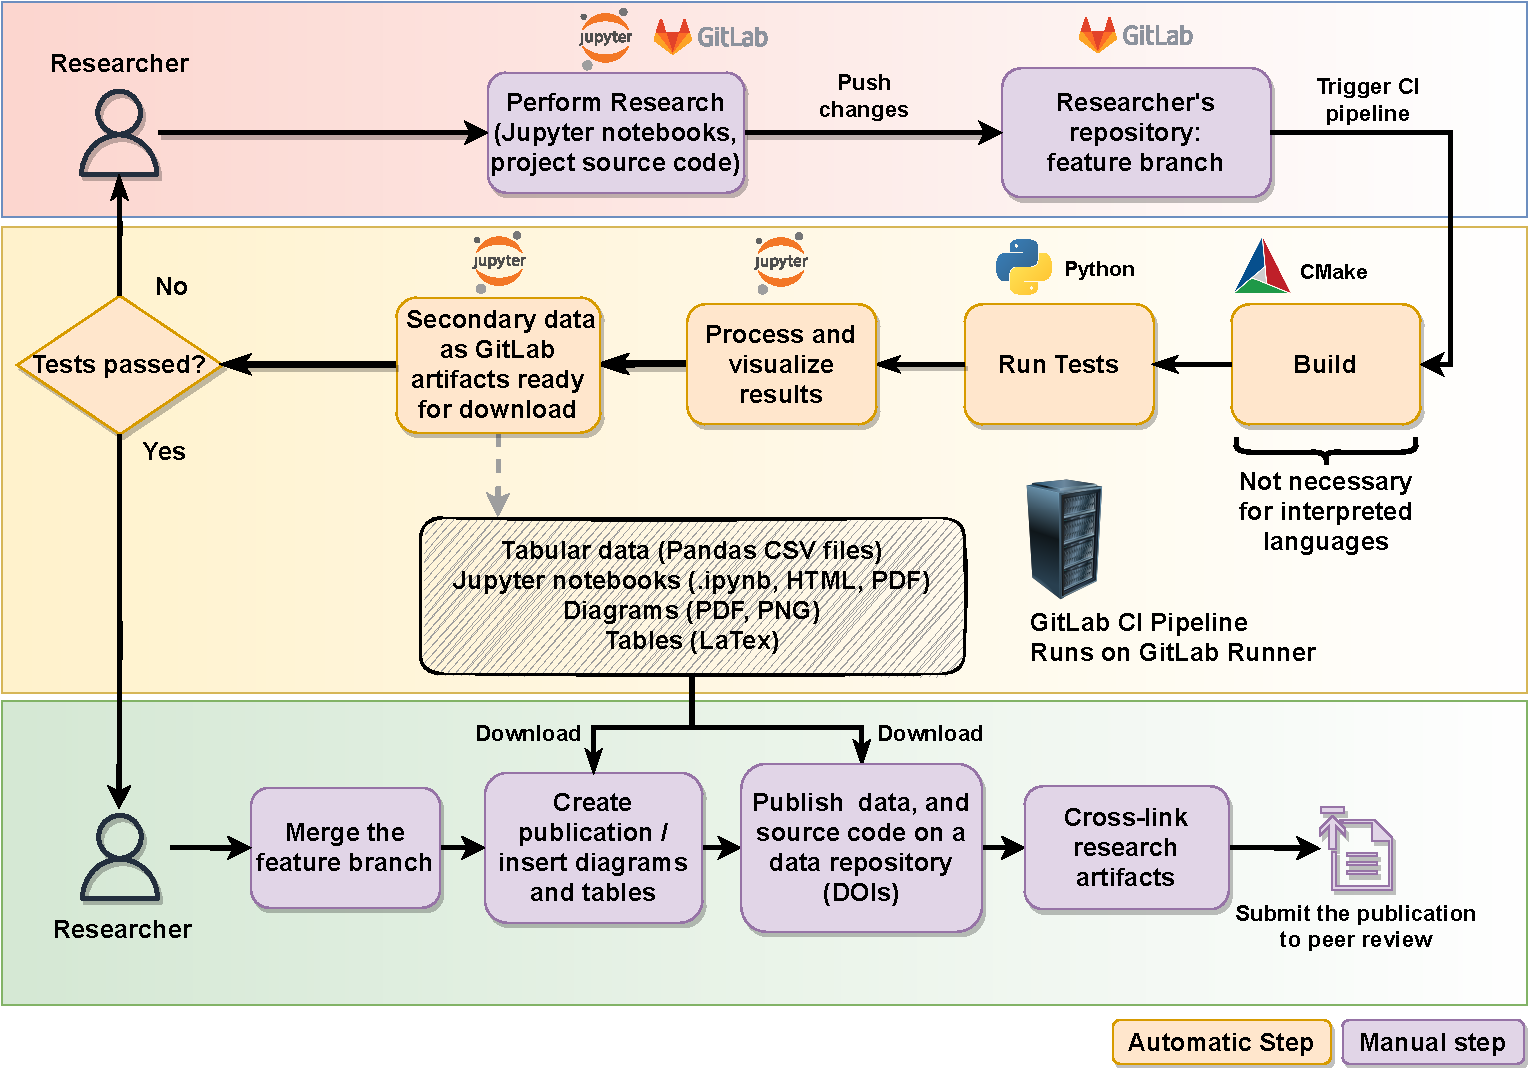
\includegraphics[width=\columnwidth]{figures/ZINF-CI-diagram-individual.pdf}
            \end{column}
            \begin{column}[c]{0.20\textwidth}
                Working alone. 
            \end{column}
        \end{columns}
\end{frame}

\begin{frame}{(Continuous) Integration of scientific software} 
\framesubtitle{CI in a nutshell I}

    \vfill

    \begin{itemize}
        \item A text (YAML) file is added to a repository, that specifies the tests (jobs) in a CI pipeline. 

        \item When the YAML file is pushed to an upstream git repository (GitLab), GitLab creates a CI pipeline from the YAML file. 

        \item The CI pipeline needs a machine to run on - the GitLab runner. 
        \item Either we install register and register our own GitLab runner, or a public one will be used.  

        \item Shared runners on gitlab.com have limited capacity. 

        \item Our Docker image must be publicly accessible for it to be used by a shared gitlab.com runner.
    \end{itemize}
\end{frame}

\begin{frame}[fragile]{(Continuous) Integration of scientific software} 
\framesubtitle{CI in a nutshell II}

    \begin{columns}
        \begin{column}[c]{0.5\textwidth}
            \begin{minted}[fontsize=\footnotesize]{yaml}
initialization_param_study:
  stage: running
  dependencies:
    - build_release
  script: 
    # run the parameter variation tests 
    - cd cases/initialization/3dinit
    - ./create_and_run_levelset.sh
    - ./reproduce_publication_results.sh
  artifacts:
    paths:
        - cases/initialization/3dinit/*.csv 
        - cases/initialization/3dinit/*.pdf 
            \end{minted}
        \end{column}
        \begin{column}[c]{0.5\textwidth}
            \begin{itemize}
                \item The GitLab CI uses a YAML file for the configuration of the CI pipeline. 
                \item The CI pipeline starts the right scripts in the right order: it documents the research workflow.
                \item A click of a button in a web browser reproduces results for any version of the research software.
                \item Continuous \emph{integration} is used to \emph{integrate} only those changes that improve the software and don't break existing tests.
            \end{itemize}
        \end{column}
    \end{columns}

\end{frame}

\begin{frame}[fragile]{(Continuous) Integration of scientific software} 
\framesubtitle{CI in a nutshell III}

    \vfill

    An example CI pipeline 
    \begin{figure}
        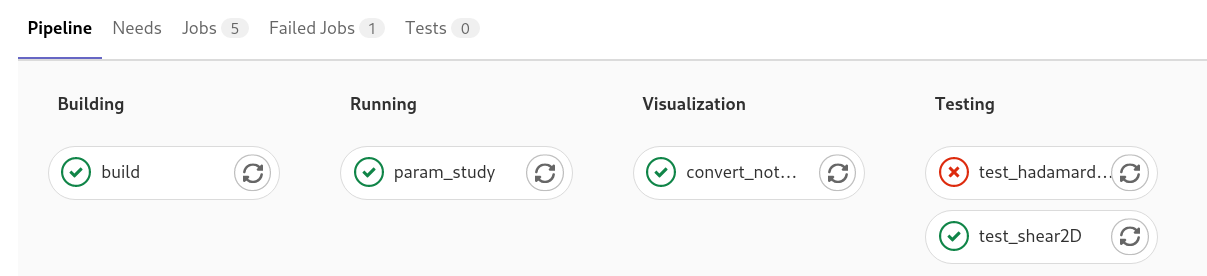
\includegraphics[width=\textwidth]{figures/pipeline-example.png}
    \end{figure}

\end{frame}

\begin{frame}{(Continuous) Integration of scientific software} 
\framesubtitle{CI in a nutshell IV}
    \vfill

    \begin{itemize}
        \item Files created within a CI job are gone when the job ends. 
        \item GitLab uses \textbf{job artifacts} to pass on data from one job to the next. 
        \item \textbf{Job artifacts can only be files stored in project's sub-folders.} 
        \item Libraries and applications are passed to other jobs as artifacts. 
        \item \textbf{Artifacts can be downloaded on the GitLab project website.}
    \end{itemize}

\end{frame}

\begin{frame}{(Continuous) Integration of scientific software} 
\framesubtitle{Running tests I}
\vfill

\begin{center}
    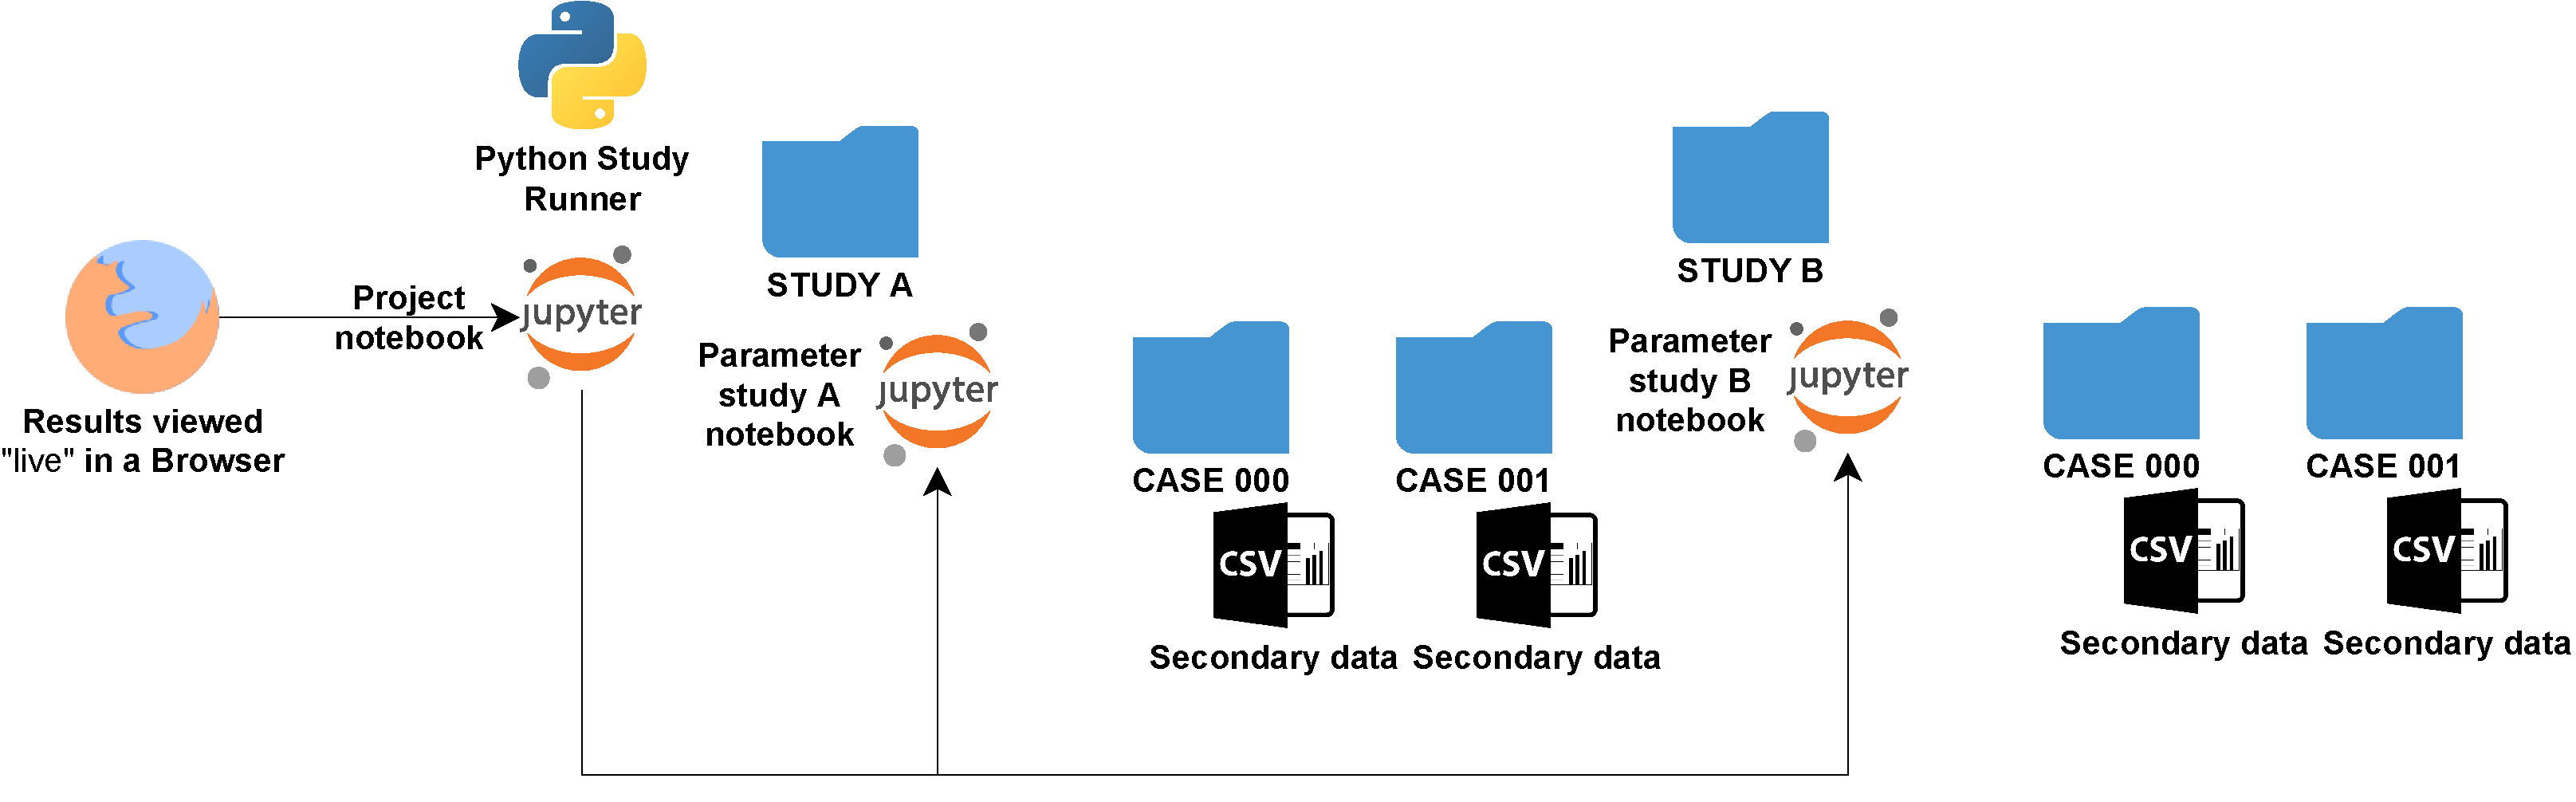
\includegraphics[width=0.9\textwidth]{figures/Cluster-Parameter-Study-Organization.pdf}
\end{center}

\end{frame}

\begin{frame}{(Continuous) Integration of scientific software} 
\framesubtitle{Running tests II}
\vfill

    \begin{itemize}
        \item Success of CSE methods is measured using verification and validation data. 
        \item Effective comparison with others (previous versions) hinges on data organization.
        \item \textbf{Goal:} being able to identify the set of study parameters used in a simulation case.
    \end{itemize}
    
    \vfill
    \begin{itemize}
        \item \textbf{Legacy code}: 
            \begin{itemize}
                \item use the existing folder structure and parameterization tools %\faGraduationCap,
                \item The mapping (case000) $\to$ (parameter vector) must be stored (YAML, ...)
            \end{itemize}
        \item \textbf{New code}: 
            \begin{enumerate}
                \item Simple folder and file structure %\faGraduationCap
                \item HDF5\footnote{\url{https://www.hdfgroup.org/solutions/hdf5}} or other open data format.
                \item Alternative to HDF5: \textbf{ExDir}\footnote{Dragly, Svenn-Arne, et al. "Experimental Directory Structure (Exdir): An alternative to HDF5 without introducing a new file format." Frontiers in neuroinformatics 12 (2018): 16.} 
            \end{enumerate}
    \end{itemize}

\end{frame}

\begin{frame}{(Continuous) Integration of scientific software} 
\framesubtitle{Running tests II}
\vfill

\begin{center}
    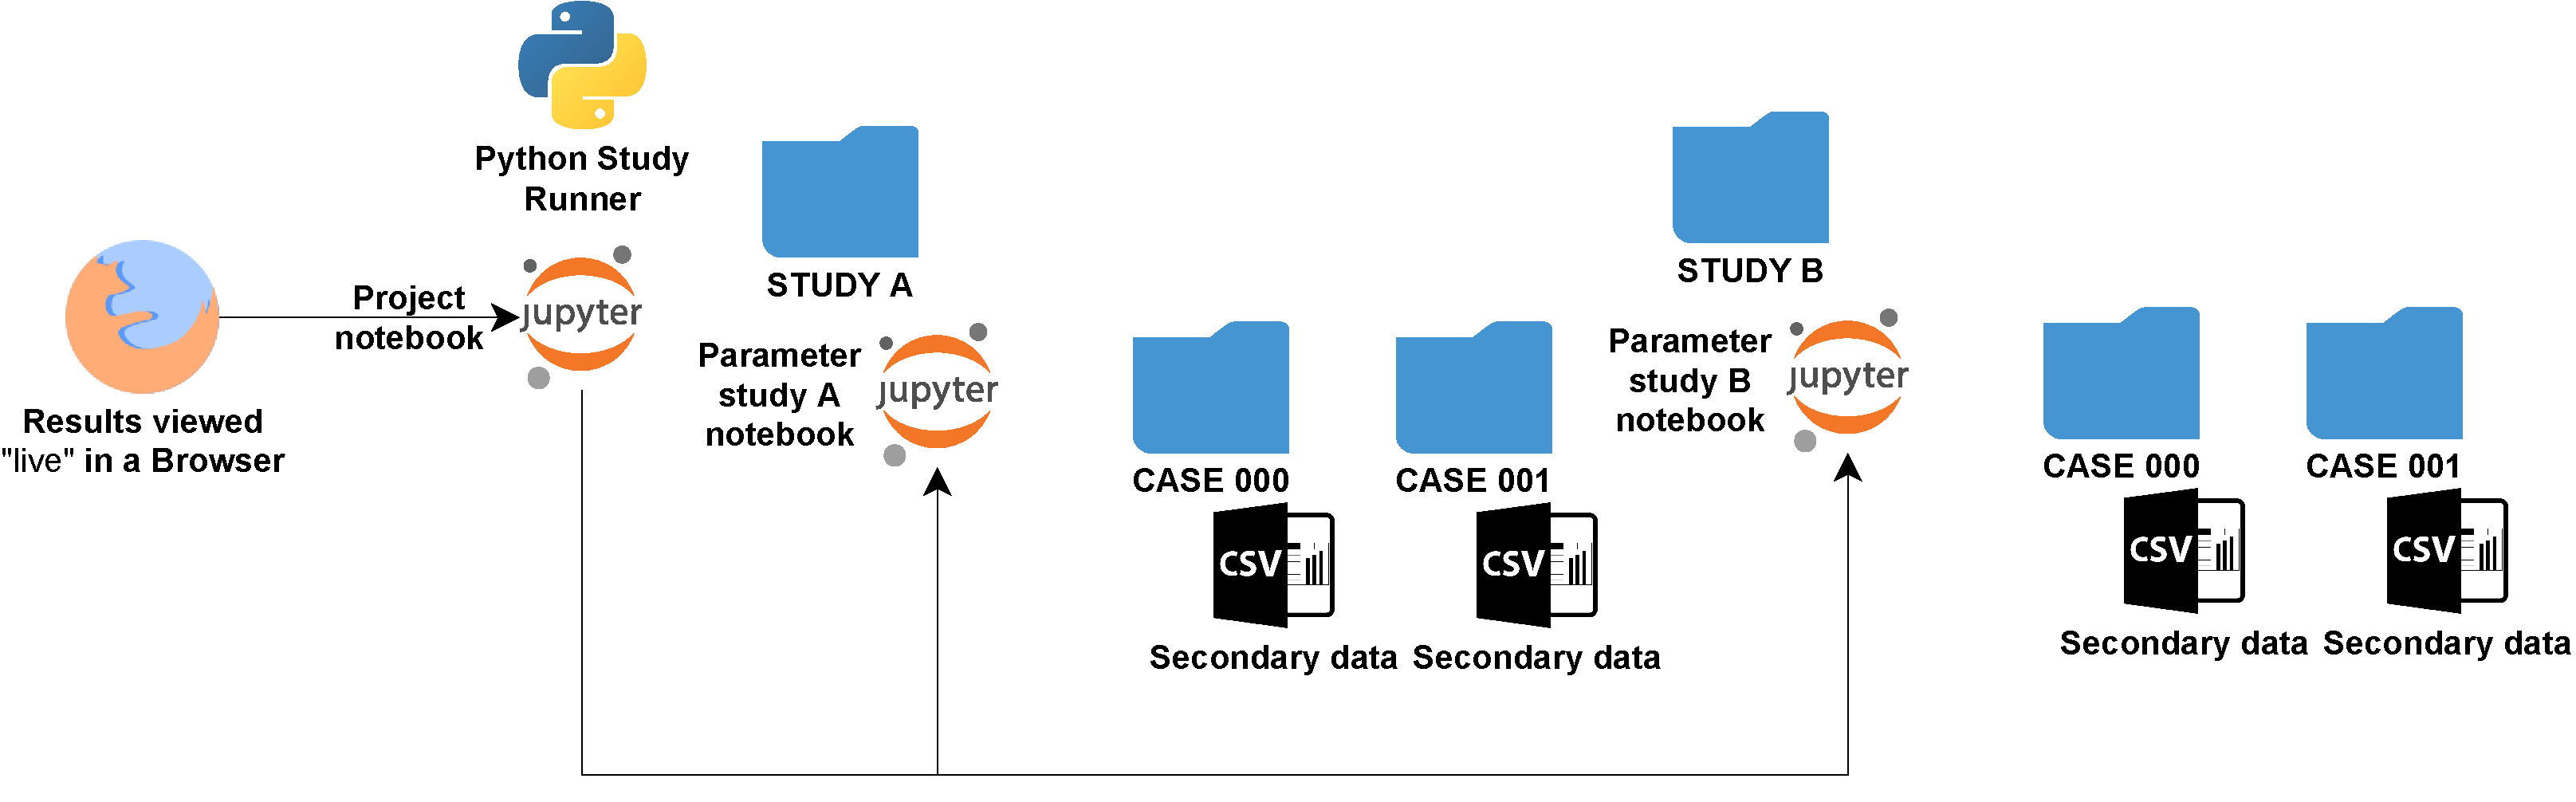
\includegraphics[width=0.9\textwidth]{figures/Cluster-Parameter-Study-Organization.pdf}
\end{center}

    \begin{itemize}
        \item Associate simulation cases with their metadata. 
        \item \texttt{\{case000 : \{N\_CELLS: 32, MODEL : shear2D\}\}}
        \item Store this information using a standard open-source format (\textbf{interoperability}).
    \end{itemize}

\end{frame}

\begin{frame}{(Continuous) Integration of scientific software} 
\framesubtitle{Running tests III}
\vfill

    Use Jupyter notebooks\footnote{\href{https://jupyter.org/}{https://jupyter.org/}} and pandas\footnote{\href{https://pandas.pydata.org/}{https://pandas.pydata.org/}} for 
    \begin{itemize}
        \item \textbf{Documentation}: geometry, initial and boundary conditions, error norms, comparison data.
        \item \textbf{Data processing}: verification errors (conservation, convergence, stability), validation errors 
        \item \textbf{Result analysis}: interactive and remote, while simulations are running!
            \begin{itemize}
                \item Jupyter notebook server can be started on a remote machine and accessed in a web browser.
            \end{itemize}
    \end{itemize}


\end{frame}

\begin{frame}{(Continuous) Integration of scientific software} 
\framesubtitle{Processing and visualizing tests}
\vfill

    \vfill

    \texttt{jupyter nbconvert notebook.ipynb --execute --to FORMAT}

    \medskip

    \begin{itemize}
        \item Agglomerate secondary data into \texttt{pandas.MultiIndex} CSV files. 
        \item Run each jupyter notebook in the repository.
        \item Export secondary data and notebooks in different formats as artifacts.
        \item \textbf{Visualization} 
            \begin{itemize}
                \item Download the artifact and open the notebook \faGraduationCap.
                \item Notebooks contain information on failing tests. 
                \item Mapping "caseID" $\to$ "parameters" is crucial for re-starting failed parameter variations! 
            \end{itemize}
    \end{itemize}

\end{frame}

\begin{frame}{(Continuous) Integration of scientific software} 
\framesubtitle{Secondary data I}
\vfill

    \begin{itemize}
        \item Data used for diagrams and tables in a publication.
        \item Data we compare our results with.
        \item Primary data: complete simulation results / experimental measurements.
    \end{itemize}

\end{frame}

\begin{frame}{(Continuous) Integration of scientific software} 
\framesubtitle{Secondary data II}
\vfill

    \href{https://pandas.pydata.org/}{pandas.MultiIndex} CSV with metadata for secondary data
    \begin{itemize}
        \item \texttt{pandas.MultiIndex} saved in "metadata columns". 
        \item \textcolor{red}{\textbf{Metadata is repeated}}: not an issue for the small secondary data! 
        \item Metadata in columns $\to$ \texttt{pandas.MultiIndex} $\to$ strongly simplified data analysis. 
        \item \textbf{Direct readable export of tables to LaTex!}
    \end{itemize}

    \footnotesize

    \begin{tabular}{llllll}
        \toprule
        {} &         H &     L\_INF &  O(L\_INF) &  EPSILON\_R\_EXACT\_MAX &  O(EPSILON\_R\_EXACT\_MAX)  \\ 
        VELOCITY\_MODEL &           &           &           &                      &                        \\ 
        \midrule
        \textcolor{red}{\textbf{SHEAR\_2D}}       &  0.125000 &  0.032961 &  1.833407 &             0.032961 &                1.833407 \\ 
        \textcolor{red}{\textbf{SHEAR\_2D}}       &  0.062500 &  0.009249 &  1.955529 &             0.009249 &                1.955529 \\ 
        \textcolor{red}{\textbf{SHEAR\_2D}}       &  0.031250 &  0.002385 &  1.988745 &             0.002385 &                1.988745 \\ 
        \textcolor{red}{\textbf{SHEAR\_2D}}       &  0.015625 &  0.000601 &  1.997178 &             0.000601 &                1.997178 \\ 
        \textcolor{red}{\textbf{SHEAR\_2D}}       &  0.007813 &  0.000150 &  1.999294 &             0.000150 &                1.999294 \\ 
        \textcolor{red}{\textbf{SHEAR\_2D}}       &  0.003906 &  0.000038 &  1.999294 &             0.000038 &                1.999294 \\ 
        \bottomrule
    \end{tabular}

\end{frame}

\begin{frame}{(Continuous) Integration of scientific software} 
\framesubtitle{Cross-linking I}
\vfill

    \begin{center}
            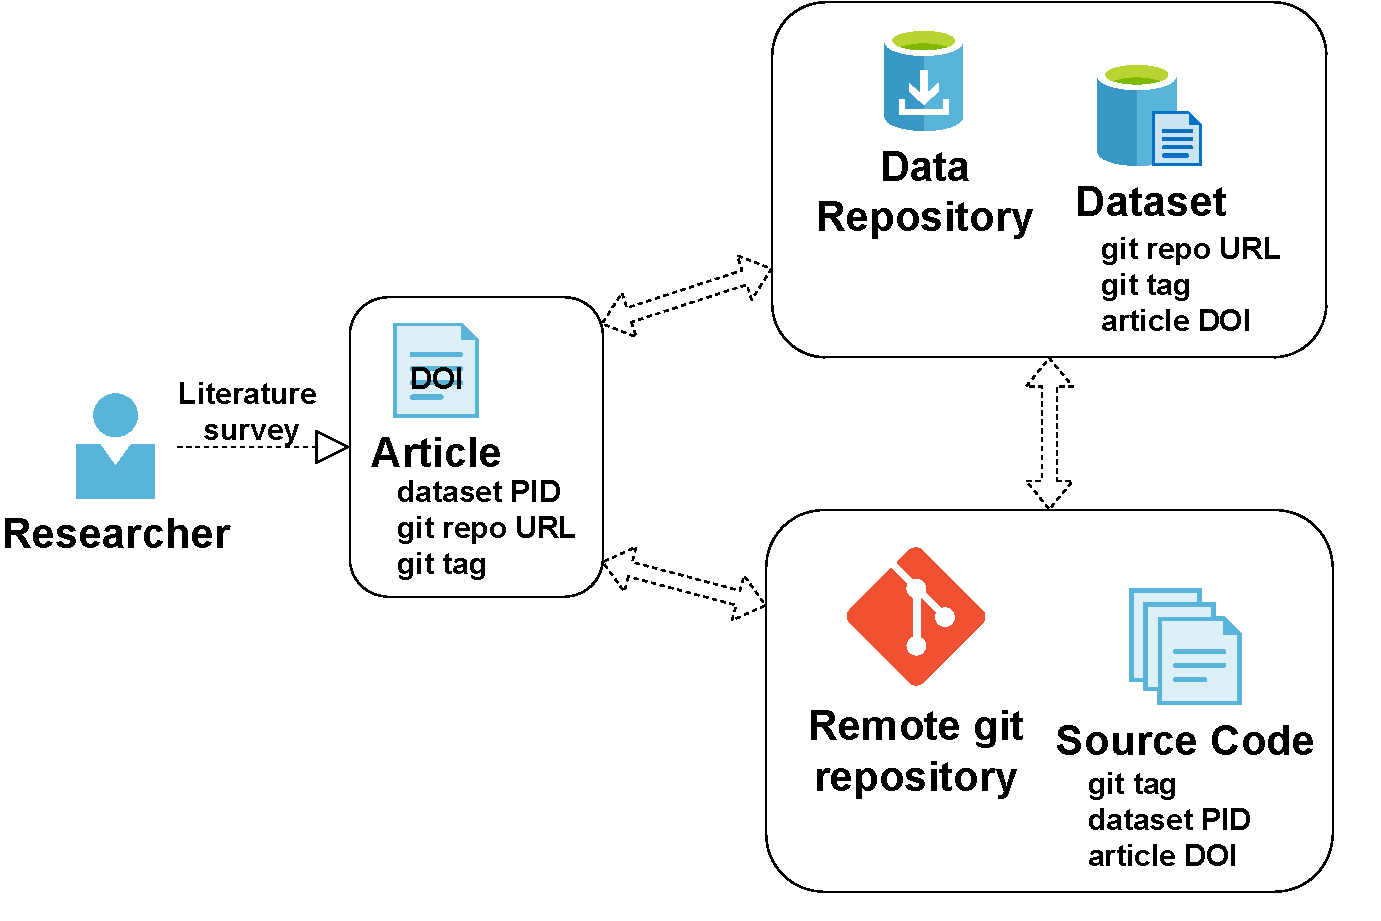
\includegraphics[width=0.67\textwidth]{figures/cross-linking.pdf}
    \end{center}

\end{frame}

\begin{frame}{(Continuous) Integration of scientific software} 
	\framesubtitle{Schematic diagram for the individual workflow}
        \vfill

        \centering

        \begin{columns}
            \begin{column}[c]{0.55\textwidth}
                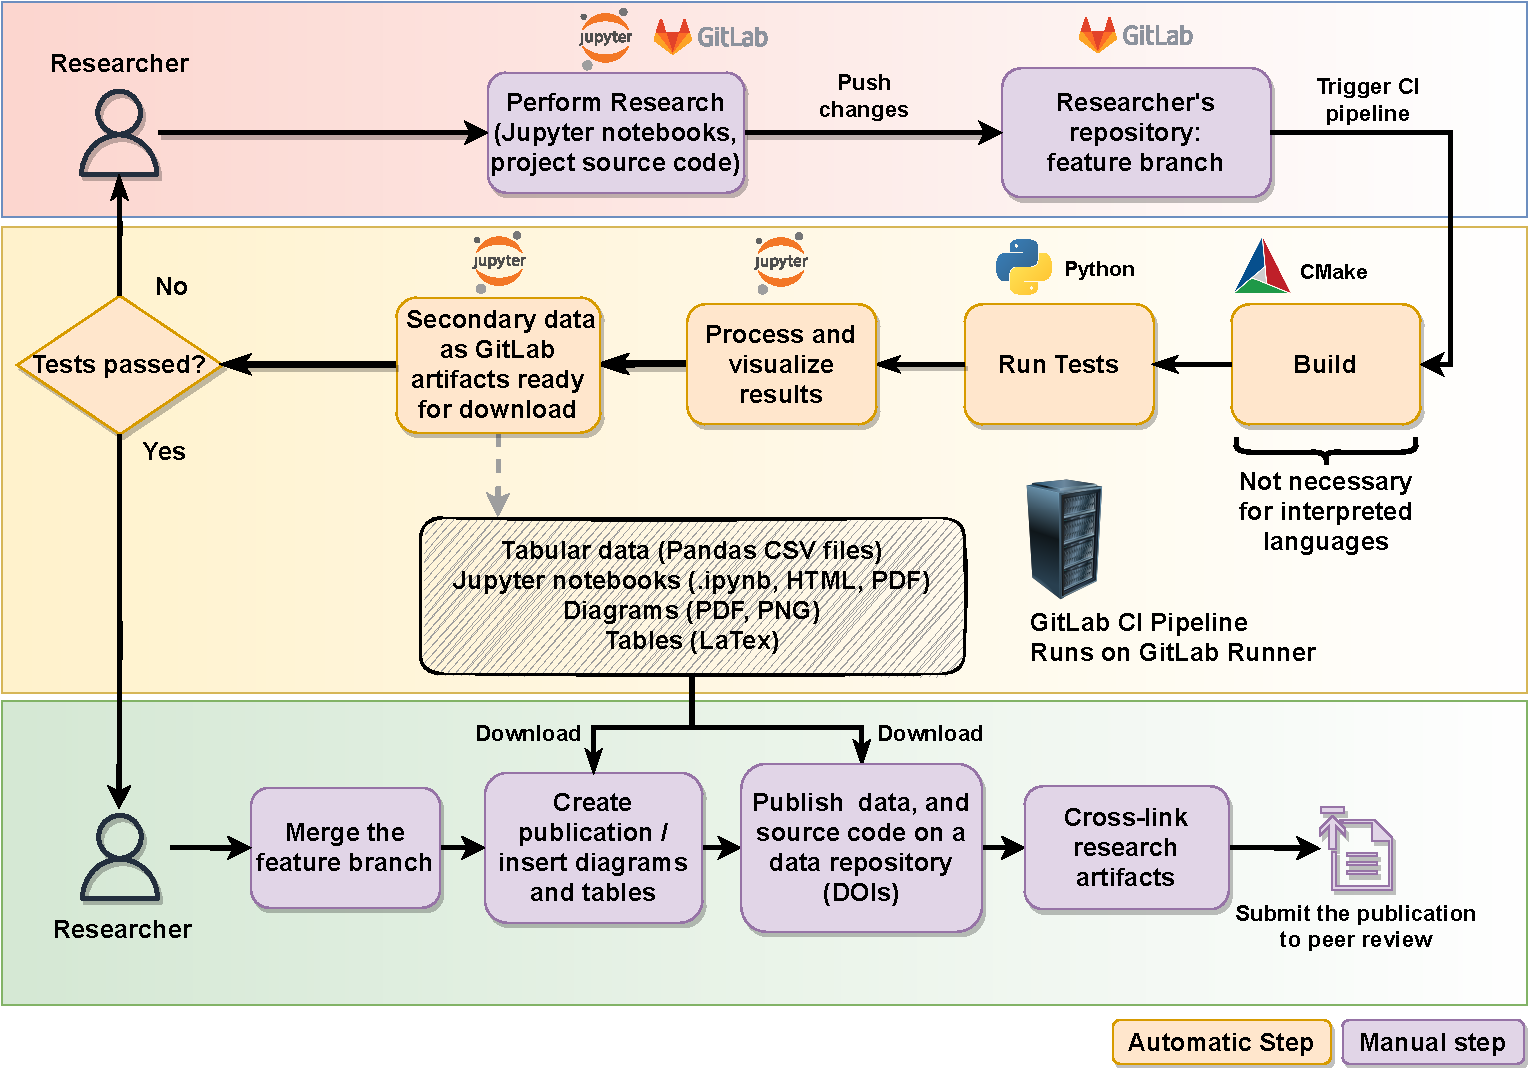
\includegraphics[width=\columnwidth]{figures/ZINF-CI-diagram-individual.pdf}
            \end{column}
            \begin{column}[c]{0.20\textwidth}
                Working alone. 
            \end{column}
        \end{columns}
\end{frame}

\begin{frame}{(Continuous) Integration of scientific software} 
\framesubtitle{Cross-linking II}
\vfill

    Cross-linking is done manually. 
    \begin{itemize}
        \item Place whatever you can under version control. 
        \item \textbf{When a set of milestones is reached (\emph{release})} , use \href{https://git-scm.com/book/en/v2/Git-Basics-Tagging}{git-tags} as version snapshots, and upload the research data to a data repository, e.g. \href{https://tudatalib.ulb.tu-darmstadt.de/}{TUDatalib} at TU Darmstadt, or \href{https://zenodo.org/}{Zenodo}.
            \begin{itemize}
                \item Secondary data (diagrams, tables), raw data (simulations, experiments), archive of the research software, ...
            \end{itemize}
        \item Data uploaded to a data repository is associated with Persistent Identifiers (PIDs), e.g. DOIs.
        \item Cite the research data using DOIs in the report (article, preprint).
        \item Upload the report to a pre-print repository, e.g. \href{https://arxiv.org/}{ArXiv}. 
        \item Edit the data on the data repository and mention the arXivID.  
        \item Submit the pre-print to a journal for peer-review.
    \end{itemize}

\end{frame}


\begin{frame}[fragile]{Continuous Integration of Scientific Software}
    \framesubtitle{Cross-linking III} 
    \vfill

    \begin{itemize}
        \item \textbf{Research software has been improved} if the results have been improved \textbf{with respect to a previous or competing publication.}
        \item A major milestone are improved results for a set of verification / validation tests.
        \item The cross-linking therefore revolves around the publication (pre-print, report, ...). 
        \item The cross-linking makes it possible to find the version of research software used to generate the results in the publication: repository link + git tag, repository snapshot, software image. 
        \item Once the version is found, CI automatically reproduces all results from the publication with a click of a button.
    \end{itemize}

\end{frame}

\begin{frame}{(Continuous Integration with result visualization)} 
    \framesubtitle{Test evaluation}

    \vfill

    Very straightforward 
    \begin{itemize}
        \item Python scripts test secondary data agglomerated by notebooks from simulation results.
        \item \textbf{Examples:} 
            \begin{itemize}
                \item Is the order of convergence of an error norm $\ge 2.0$?
                \item Is is the difference between simulation and experiment data $\le 4\%$? 
            \end{itemize}
    \end{itemize}

\end{frame}


\begin{frame}{(Continuous) Integration of scientific software} 
    \framesubtitle{Docker (containerization)}
    \vfill

    \begin{columns}
        \begin{column}[c]{0.4\textwidth}
            \begin{center}
            \only<1>{
                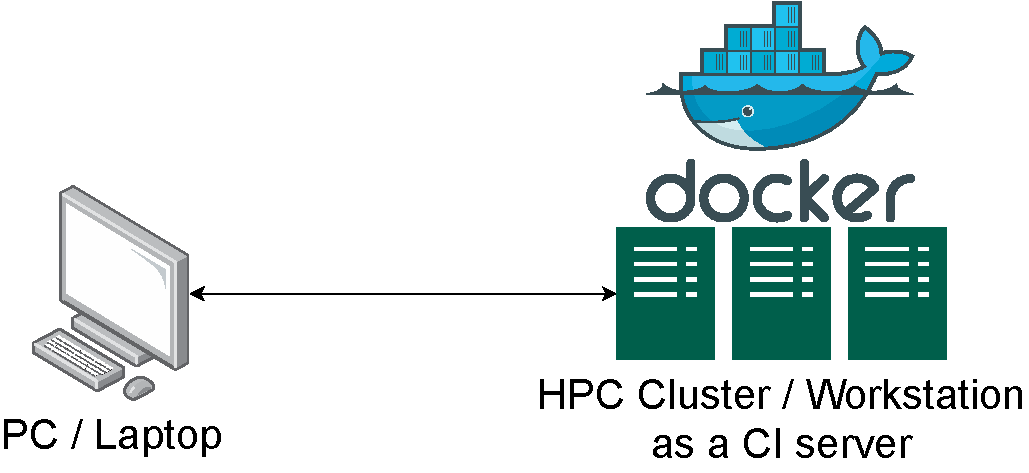
\includegraphics[width=\columnwidth]{figures/ci-with-docker.pdf}
            }
            \only<2>{
                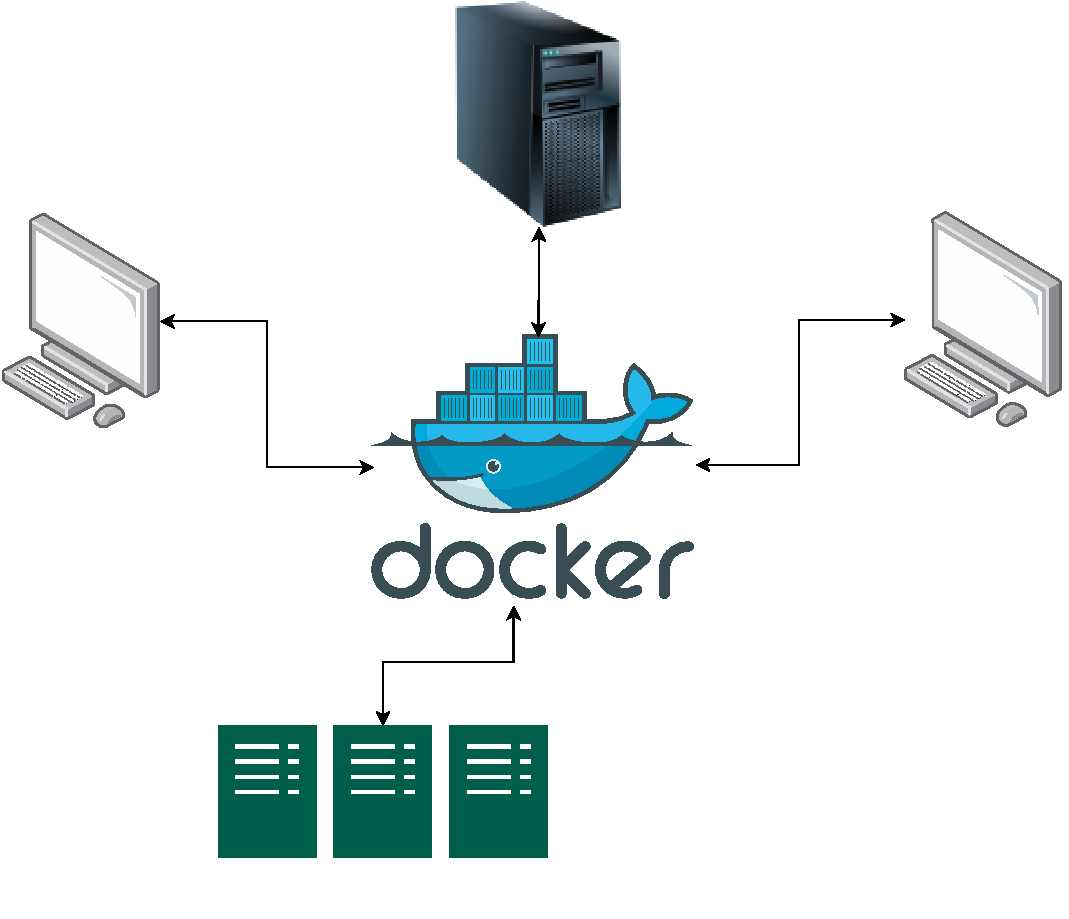
\includegraphics[width=\columnwidth]{figures/docker-description.pdf}
            }
            \end{center}
        \end{column}
        \begin{column}[c]{0.6\textwidth}
            \begin{itemize}
                \item Instead of installing the research software only on the laptop/PC and the HPC cluster / workstation, we install it in a virtual environment - \textbf{a Docker image}.
                \item The Docker image then works on any machine that runs Docker. 
                \item Sharing research software becomes trivial - if our colleague wants to use our software, no installation (besides Docker) is required. 
            \end{itemize}
        \end{column}
    \end{columns}

\end{frame}

\begin{frame}{(Continuous) Integration of scientific software} 
\framesubtitle{Computing resources}
\vfill

    \vfill
    The GitLab CI requires a \textbf{GitLab runner: a machine that runs the CI jobs.}
    \begin{enumerate}
        \item \textbf{Short few CPU-core tests}: work-PC \faGraduationCap.    
        \item \textbf{Short many-core tests}: obtain a workstation with a 64-Core CPU\footnote{Thanks to \href{https://www.sfb1194.tu-darmstadt.de/index.en.jsp}{CRC 1194 at TU Darmstadt.}}\faGraduationCap.
        \item \textbf{HPC tests}: combine 1. or 2. with an HPC cluster. 
    \end{enumerate}

    An HPC cluster is relevant for production tests and performance measurements.
    \begin{itemize}
        \item This workflow uses coarse ("smoke") tests \faGraduationCap
            \begin{itemize}
                \item Unit tests run for 1. and 2.
                \item Convergence ensured for 1. and 2.
                \item Is efficient in parallel for 1. and 2. 
            \end{itemize}
        \item \textbf{Challenge}: Is it possible to combine 1., 2. and 3. and publish instead of perish \faGraduationCap?
    \end{itemize}

\end{frame}

%\begin{frame}{(Continuous) Integration of scientific software} 
    %\framesubtitle{A GitLab runner with a Docker executor and a local Docker image}

    %\vfill 
    %Build a Docker image for your software, and track the Dockerfile with the project.\\
    %\medskip
    %\href{https://gitlab.com/tmaric/fvc-reconstruct/-/tree/main/docker}{Example OpenFOAM Dockerfile} on \texttt{ubuntu:focal} with "system" open-mpi and scotch.

    %\medskip
    %On the testing machine
    %\begin{itemize}
        %\item Install Docker and GitLab runner and register the GitLab runner with a Docker executor.
        %\item Configure the GitLab runner in \texttt{/etc/gitlab-runner/config.toml} to
            %\begin{itemize}
                %\item use a local Docker image, e.g., \texttt{image = "openfoam-v2012\_ubuntu-focal:latest"}, and
                %\item never pull images \texttt{pull\_policy = never}.
            %\end{itemize}
    %\end{itemize}

%\end{frame}

\begin{frame}{(Continuous) Integration of scientific software} 
    \framesubtitle{Summary}

\begin{columns}
    \begin{column}[c]{0.51\textwidth}
        \centering
        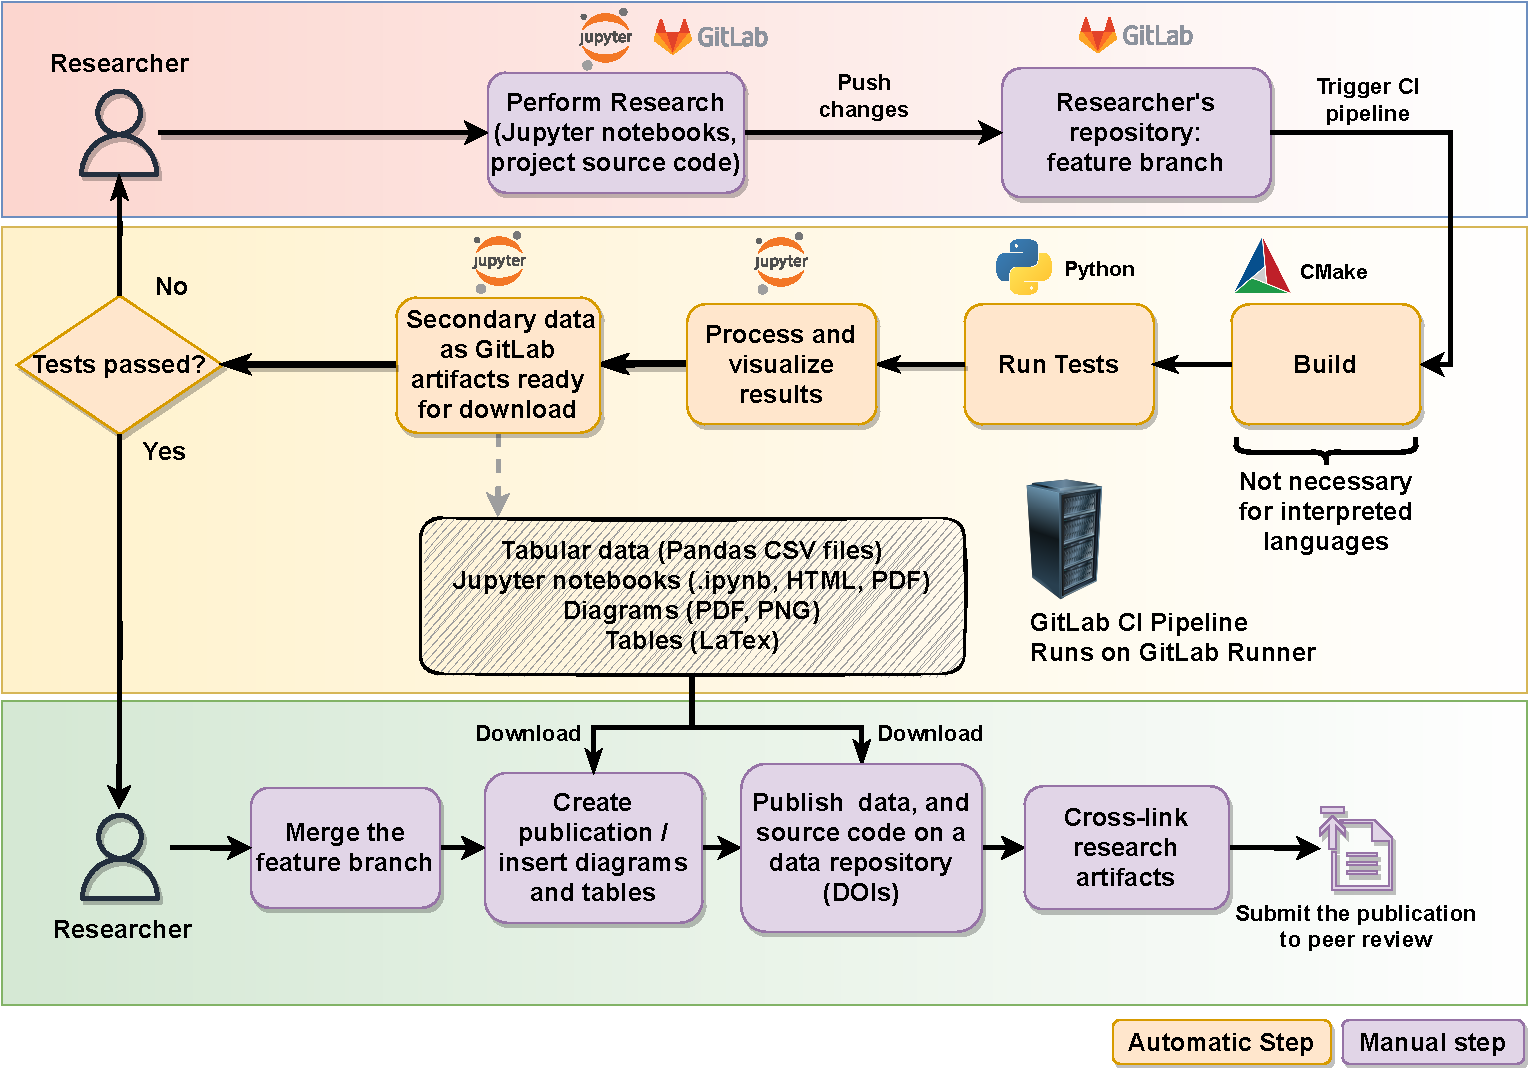
\includegraphics[width=\columnwidth]{figures/ZINF-CI-diagram-individual.pdf}
    \end{column}
    \begin{column}[c]{0.49\textwidth}
        \footnotesize
        \begin{algorithmic}[1]
            \State Track changes using version-control.
            \While{Milestone not reached}
                \For{study in studies} \Comment On an HPC cluster.
                    \State Automate data processing and visualization.
                    \State Run study.
                    \State Check results and apply code changes. 
                \EndFor
                \If{results are improved on the HPC cluster} 
                    \State Push changes to the remote repository. 
                    \If{CI pipeline tests pass}
                        \State Milestone reached.
                        \State Add new tests to the CI pipeline, 
                        \State Merge feature into development branch. 
                        \State Cross-link publication, data, and source code.
                    \EndIf
                \EndIf
            \EndWhile
        \end{algorithmic}
    \end{column}
\end{columns}

\end{frame}

\begin{frame}{(Continuous) Integration of scientific software} 
\framesubtitle{Similarity with other workflows / best practices}

	\vfill
	Our \emph{(subjective)} estimates* of similarity $1-5$ (higher is more similar), $-$: aspect not addressed.
	\begin{center}
		\scriptsize
		\begin{tabular}{@{} *6l @{}}    \toprule
				\emph{DOI} & \emph{Branching model} & \emph{TDD} & \emph{Cross-linking} & \emph{CI}  & (Meta)data standardization \\\midrule
				 \href{https://doi.org/10.12688/f1000research.11407.1}{10.12688/f1000research.11407.1} 
					 & -  & -  & -  & - & 1  \\ 
				 \href{https://doi.org/10.3934/math.2016.3.261}{10.3934/math.2016.3.261} 
					 & -  & -  & -  & - & 2  \\ 
				 \href{https://doi.org/10.1371/journal.pbio.1001745}{10.1371/journal.pbio.1001745} 
					 & 1  & 2  & -  & - & -  \\ 
				 \href{https://doi.org/10.1371/journal.pcbi.1005510}{10.1371/journal.pcbi.1005510}
					 & -  & -  & 3 & 1 & 3  \\ 
				 \href{https://doi.org/10.1145/2723872.2723881}{10.1145/2723872.2723881}
					 & 1  & -  & - & 1 & -  \\ 
				 \href{https://dl.acm.org/doi/10.1145/3324989.3325719}{10.1145/3324989.3325719}
					 & 1  & -  & - & 5 & -  \\ 
				 \href{https://doi.org/10.1371/journal.pone.0230557}{10.1371/journal.pone.0230557}
					 & 1  & -  & - & 1 & 4  \\ 
				 \href{https://doi.org/10.1145/3219104.3219147}{10.1145/3219104.3219147} 
					 & 1  & -  & -  & 4 & - \\\bottomrule
				 \hline
		\end{tabular}
	\end{center}
	
	*\emph{The list may still be incomplete.}
	
\end{frame}

%\begin{frame}[fragile]{(Continuous Integration with result visualization)} 
    %\framesubtitle{Building OpenFOAM projects or projects with out-of-source installation}

    %\vfill
    %\textbf{Out-of-source installation}: binaries only available outside the repo! 
    %\begin{itemize}
        %\item \textbf{Use environment variables to build and pass on artifacts} 
        %\item \texttt{\$FOAM\_USER\_LIBBIN} folder stores library binaries. 
        %\item \texttt{\$FOAM\_USER\_APPBIN} folder stores application binaries. 
        %\item \textbf{Build job}: 
            %\begin{itemize}
                %\item create artifact folders inside the repo, 
                %\item copy library and application binaries to artifact folders, 
                %\item export artifact folders. 
            %\end{itemize}
        %\item \textbf{Run job: \textbf{simplified} copying of binary artifacts to OpenFOAM folders}
            %\begin{itemize} 
                %\item \texttt{mkdir -p} \texttt{\{\$FOAM\_USER\_LIBBIN, \$FOAM\_USER\_APPBIN\}}
                %\item \texttt{cp FOAM\_USER\_LIBBIN/* \$FOAM\_USER\_LIBBIN} 
                %\item \texttt{cp FOAM\_USER\_APPBIN/* \$FOAM\_USER\_APPBIN} 
                %\item Run tests.
            %\end{itemize}
    %\end{itemize}


%\end{frame}


%\begin{frame}{(Continuous Integration with result visualization)} 
    %\framesubtitle{Example}

    %\vfill
    %\begin{center}
        %\href{https://gitlab.com/tmaric/fvc-reconstruct/-/pipelines/279564790}{Example OpenFOAM CI project} 
    %\end{center}

%\end{frame}

\section{Continuous Integration hands-on}

\begin{frame}
\end{frame}


\begin{frame}{Summary: the minimal workflow} 
    \vfill

    Minimal workflow
    \begin{itemize}
        \item Track the status of your project using the GitLab Kanban board.
        \item Learn and apply the very basics of git, understand the concepts behind branching, merging, commits and working with remote repositories.   
        \item Integrate the changes that worked, don't leave 30 branches open. 
        \item Format the data using established (open-source) formats if possible, if not, at least do this for secondary data (diagrams and tables). 
        \item Share your secondary data on a (TUdatalib) data repository. 
        \item Periodically cross-link research data: publication/report, scripts/code, secondary and primary data. 
    \end{itemize}

\end{frame}


%\begin{frame}{Lessons learned}
	%\vfill
        %\begin{itemize}
            %\item Keeping the workflow as simple as possible is crucial for acceptance.
            %\item Focusing on secondary data simplifies the workflow significantly.  
            %\item For simulations that run $<24$ hours primary data can be recomputed easily. 
            %\item Periodical cross-linking of research data is done quickly and it is very beneficial. 
            %\item Personal responsibility is crucial at University research groups: who are the maintainers? 
                %\begin{itemize}
                    %\item What are the incentives for maintainers? 
                %\end{itemize}
            %\item Fixing the (parallel) I/O of legacy scientific codes requires a large amount of effort. 
                %\begin{itemize}
                    %\item It should be done outside of research projects. 
                %\end{itemize}
        %\end{itemize}
%\end{frame}

%\begin{frame}{Outlook}
	%\vfill
	%\begin{itemize}
            %\item Performance CI jobs run on 64-core workstations: moving on to the HPC cluster. 
            %\item Singularity GitLab executor? 
            %\item Jupyter Hub for interactive analysis of problems in parameter variations?
            %\item Automatic publishing and cross-linking of CI artifacts? 
                %\begin{itemize}
                    %\item Source code archive, Singularity container, secondary data. 
                    %\item Data repository API must be used to modify metadata. 
                %\end{itemize}
	%\end{itemize}
%\end{frame}




\begin{frame}{Acknowledgements}

    \vfill
    \begin{center}
        
\includegraphics[width=0.5\textwidth]{crc-logo}
    \end{center}
    \begin{center}
        Funded by the German Research Foundation (DFG) – Project-ID 265191195 – \href{https://www.sfb1194.tu-darmstadt.de/index.en.jsp}{CRC 1194} : Z-INF
    \end{center}

\end{frame}

\end{document}

